% This is the Amherst College Thesis and Comprehensive Evaluation
% LaTeX template. Brittney E. Bailey adapted this template from the
% Reed College LaTeX thesis template in January 2019. Most of the work
% for the document class was done by Sam Noble (SN), as well as this
% template. Later comments etc. by Ben Salzberg (BTS). Additional
% restructuring and APA support by Jess Youngberg (JY).
% Your comments and suggestions are more than welcome; please email
% them to cus@reed.edu
%
% See http://web.reed.edu/cis/help/latex.html for help. There are a
% great bunch of help pages there, with notes on
% getting started, bibtex, etc. Go there and read it if you're not
% already familiar with LaTeX.
%
% Any line that starts with a percent symbol is a comment.
% They won't show up in the document, and are useful for notes
% to yourself and explaining commands.
% Commenting also removes a line from the document;
% very handy for troubleshooting problems. -BTS

%%
%% Preamble
%%
% \documentclass{<something>} must begin each LaTeX document
\documentclass[12pt,twoside]{amherstthesis}
% Packages are extensions to the basic LaTeX functions. Whatever you
% want to typeset, there is probably a package out there for it.
% Chemistry (chemtex), screenplays, you name it.
% Check out CTAN to see: http://www.ctan.org/
%%
\usepackage{graphicx,latexsym}
\usepackage{amsmath}
\usepackage{amssymb,amsthm}
\usepackage{longtable,booktabs,setspace}
\usepackage{chemarr} %% Useful for one reaction arrow, useless if you're not a chem major
\usepackage[hyphens]{url}
% Added by CII
\usepackage{hyperref}
\usepackage{lmodern}
\usepackage{float}
\floatplacement{figure}{H}
% End of CII addition
\usepackage{rotating}

% Next line commented out by CII
%%% \usepackage{natbib}
% Comment out the natbib line above and uncomment the following two lines to use the new
% biblatex-chicago style, for Chicago A. Also make some changes at the end where the
% bibliography is included.
%\usepackage{biblatex-chicago}
%\bibliography{thesis}


% Added by CII (Thanks, Hadley!)
% Use ref for internal links
\renewcommand{\hyperref}[2][???]{\autoref{#1}}
\def\chapterautorefname{Chapter}
\def\sectionautorefname{Section}
\def\subsectionautorefname{Subsection}
% End of CII addition
\usepackage{xcolor}
\hypersetup{
    colorlinks,
    linkcolor={red!50!black},
    citecolor={blue!50!black},
    urlcolor={blue!80!black}
}
% Added by CII
\usepackage{caption}
\captionsetup{width=5in}
% End of CII addition

\usepackage{titlesec}

% \titleformat{⟨command⟩}[⟨shape⟩]{⟨format⟩}{⟨label⟩}{⟨sep⟩}{⟨before-code⟩}[⟨after-code⟩]
\titleformat{\chapter}[hang]
{\normalfont%
    \Large% %change this size to your needs for the first line
    \bfseries}{\chaptertitlename\ \thechapter}{20pt}{%
     %change this size to your needs for the second line
    }[]

\titleformat{\section}[hang]
{\normalfont%
    \large % %change this size to your needs for the first line
    \bfseries}{\thesection}{20pt}{%
     %change this size to your needs for the second line
    }[]

\titleformat{\subsection}[hang]
{\normalfont%
    \normalsize % %change this size to your needs for the first line
    \bfseries}{\thesubsection}{15pt}{%
     %change this size to your needs for the second line
    }[]

% \titleformat{\section}[display]
% {\normalfont%
%     \large% %change this size to your needs for the first line
%     \bfseries}{\chaptertitlename\ \thechapter}{20pt}{%
%     \normalsize %change this size to your needs for the second line
%     }

% \usepackage{times} % other fonts are available like times, bookman, charter, palatino

% Syntax highlighting #22
  \usepackage{color}
  \usepackage{fancyvrb}
  \newcommand{\VerbBar}{|}
  \newcommand{\VERB}{\Verb[commandchars=\\\{\}]}
  \DefineVerbatimEnvironment{Highlighting}{Verbatim}{commandchars=\\\{\}}
  % Add ',fontsize=\small' for more characters per line
  \usepackage{framed}
  \definecolor{shadecolor}{RGB}{248,248,248}
  \newenvironment{Shaded}{\begin{snugshade}}{\end{snugshade}}
  \newcommand{\KeywordTok}[1]{\textcolor[rgb]{0.13,0.29,0.53}{\textbf{#1}}}
  \newcommand{\DataTypeTok}[1]{\textcolor[rgb]{0.13,0.29,0.53}{#1}}
  \newcommand{\DecValTok}[1]{\textcolor[rgb]{0.00,0.00,0.81}{#1}}
  \newcommand{\BaseNTok}[1]{\textcolor[rgb]{0.00,0.00,0.81}{#1}}
  \newcommand{\FloatTok}[1]{\textcolor[rgb]{0.00,0.00,0.81}{#1}}
  \newcommand{\ConstantTok}[1]{\textcolor[rgb]{0.00,0.00,0.00}{#1}}
  \newcommand{\CharTok}[1]{\textcolor[rgb]{0.31,0.60,0.02}{#1}}
  \newcommand{\SpecialCharTok}[1]{\textcolor[rgb]{0.00,0.00,0.00}{#1}}
  \newcommand{\StringTok}[1]{\textcolor[rgb]{0.31,0.60,0.02}{#1}}
  \newcommand{\VerbatimStringTok}[1]{\textcolor[rgb]{0.31,0.60,0.02}{#1}}
  \newcommand{\SpecialStringTok}[1]{\textcolor[rgb]{0.31,0.60,0.02}{#1}}
  \newcommand{\ImportTok}[1]{#1}
  \newcommand{\CommentTok}[1]{\textcolor[rgb]{0.56,0.35,0.01}{\textit{#1}}}
  \newcommand{\DocumentationTok}[1]{\textcolor[rgb]{0.56,0.35,0.01}{\textbf{\textit{#1}}}}
  \newcommand{\AnnotationTok}[1]{\textcolor[rgb]{0.56,0.35,0.01}{\textbf{\textit{#1}}}}
  \newcommand{\CommentVarTok}[1]{\textcolor[rgb]{0.56,0.35,0.01}{\textbf{\textit{#1}}}}
  \newcommand{\OtherTok}[1]{\textcolor[rgb]{0.56,0.35,0.01}{#1}}
  \newcommand{\FunctionTok}[1]{\textcolor[rgb]{0.00,0.00,0.00}{#1}}
  \newcommand{\VariableTok}[1]{\textcolor[rgb]{0.00,0.00,0.00}{#1}}
  \newcommand{\ControlFlowTok}[1]{\textcolor[rgb]{0.13,0.29,0.53}{\textbf{#1}}}
  \newcommand{\OperatorTok}[1]{\textcolor[rgb]{0.81,0.36,0.00}{\textbf{#1}}}
  \newcommand{\BuiltInTok}[1]{#1}
  \newcommand{\ExtensionTok}[1]{#1}
  \newcommand{\PreprocessorTok}[1]{\textcolor[rgb]{0.56,0.35,0.01}{\textit{#1}}}
  \newcommand{\AttributeTok}[1]{\textcolor[rgb]{0.77,0.63,0.00}{#1}}
  \newcommand{\RegionMarkerTok}[1]{#1}
  \newcommand{\InformationTok}[1]{\textcolor[rgb]{0.56,0.35,0.01}{\textbf{\textit{#1}}}}
  \newcommand{\WarningTok}[1]{\textcolor[rgb]{0.56,0.35,0.01}{\textbf{\textit{#1}}}}
  \newcommand{\AlertTok}[1]{\textcolor[rgb]{0.94,0.16,0.16}{#1}}
  \newcommand{\ErrorTok}[1]{\textcolor[rgb]{0.64,0.00,0.00}{\textbf{#1}}}
  \newcommand{\NormalTok}[1]{#1}

% To pass between YAML and LaTeX the dollar signs are added by CII
\title{Wines Around the World}
\author{YZ Analytics}
% The month and year that you submit your FINAL draft TO THE LIBRARY (May or December)
\date{December 11, 2019}
%\division{}
%\advisor{}
%\institution{Amherst College}
%\degree{}
%If you have two advisors for some reason, you can use the following
% Uncommented out by CII
% End of CII addition

%%% Remember to use the correct department!
%\department{}
% if you're writing a thesis in an interdisciplinary major,
% uncomment the line below and change the text as appropriate.
% check the Senior Handbook if unsure.
%\thedivisionof{The Established Interdisciplinary Committee for}
% if you want the approval page to say "Approved for the Committee",
% uncomment the next line
%\approvedforthe{Committee}

% Added by CII
%%% Copied from knitr
%% maxwidth is the original width if it's less than linewidth
%% otherwise use linewidth (to make sure the graphics do not exceed the margin)
\makeatletter
\def\maxwidth{ %
  \ifdim\Gin@nat@width>\linewidth
    \linewidth
  \else
    \Gin@nat@width
  \fi
}
\makeatother

\renewcommand{\contentsname}{Table of Contents}
% End of CII addition

\setlength{\parskip}{0pt}

% Added by CII

\providecommand{\tightlist}{%
  \setlength{\itemsep}{0pt}\setlength{\parskip}{0pt}}

\Acknowledgements{

}

\Dedication{

}

\Preface{

}

\Abstract{

}

% End of CII addition
%%
%% End Preamble
%%
%
\begin{document}

\doublespace
% Everything below added by CII
  \maketitle

\frontmatter % this stuff will be roman-numbered

\pagenumbering{roman}
\pagestyle{fancyplain}
%\pagestyle{fancy} % this removes page numbers from the frontmatter






  \hypersetup{linkcolor=black}
  \setcounter{tocdepth}{2}
  \tableofcontents

% % \addcontentsline{toc}{chapter}{List of Tables}\listoftables
%
% % \addcontentsline{toc}{chapter}{List of Figures}\listoffigures
%

\mainmatter % here the regular arabic numbering starts
\pagenumbering{arabic}
\pagestyle{fancyplain} % turns page numbering back on

\chapter*{Introduction}\label{introduction}
\addcontentsline{toc}{chapter}{Introduction}

The first traces of wine were found in Georgia in 6000BCE\footnote{Watson
  (2010)}. In \textbf{Figure 1} we show a map of more than 10 thousand
wineries operational today.
\begin{figure}[htbp]
\centering
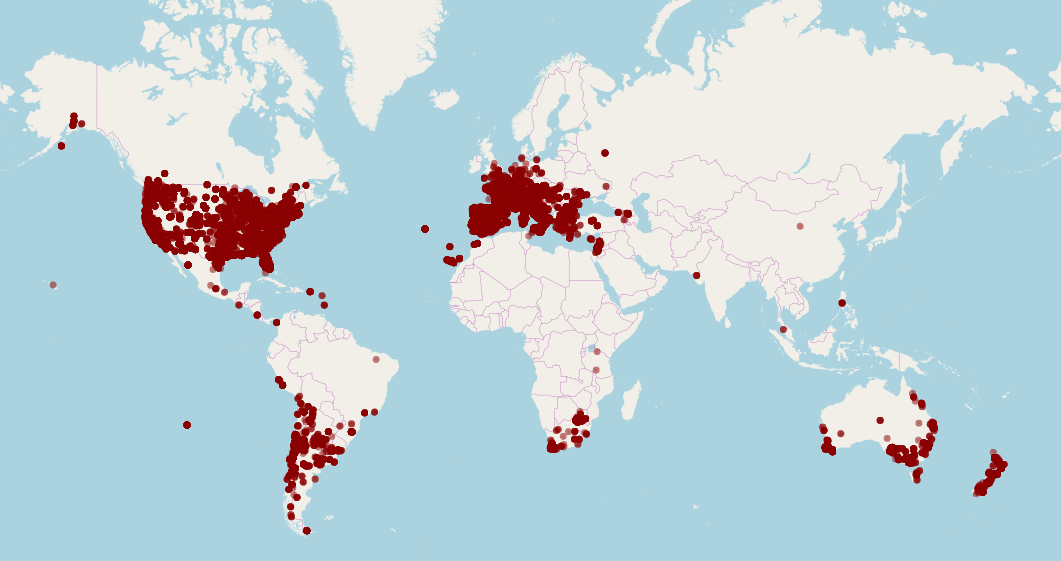
\includegraphics[width=0.8\columnwidth]{../assets/wineries.png}
\caption{Map of more than 10000 wineries present in our dataset.}
\end{figure}
For more than 8000 years, wine has been a relevant part of civilization,
and yet, many people still do not think twice when they say ``I'm not a
wine person''. Even then, there are many people that are also able to
comfortably say: ``This juicy, fruit-forward wine delectates the
palate.''

This report and the accompanying
\href{https://szablah.shinyapps.io/wine/}{web application} aim for two
things: 1) to showcase an advanced usage of visualization techniques in
the context of a product for wine exploration, and 2) to expand and
develop statistical techniques for a seamless incorporation into our
product. Therefore, our main goal is to provide an immersive experience
which leverages technology and builds upon the statistical/technical
knowledge of a bachelor-level student, all within the context of wine.

\section{Data Provenance}\label{data-provenance}

In this project we will be working with Kaggle's wine review data, found
\href{https://www.kaggle.com/zynicide/wine-reviews}{here}\footnote{Thoutt
  (2017)}. There are close to 130,000 wine reviews from
\href{https://www.winemag.com/?s=\&drink_type=wine\&page=0}{Wine
Magazine's website}\footnote{(``Wine enthusiast reviews,'' 2019)}. A
small glimpse of what the data looks like is available below for
convenience:
\begin{verbatim}
     Observations: 129,971
     Variables: 14
     $ X1                    <dbl> 0, 1, 2, 3, 4, 5, 6, 7, 8, 9, 10, 11, 12...
     $ country               <chr> "Italy", "Portugal", "US", "US", "US", "...
     $ description           <chr> "Aromas include tropical fruit, broom, b...
     $ designation           <chr> "Vulkà Bianco", "Avidagos", NA, "Reserve...
     $ points                <dbl> 87, 87, 87, 87, 87, 87, 87, 87, 87, 87, ...
     $ price                 <dbl> NA, 15, 14, 13, 65, 15, 16, 24, 12, 27, ...
     $ province              <chr> "Sicily & Sardinia", "Douro", "Oregon", ...
     $ region_1              <chr> "Etna", NA, "Willamette Valley", "Lake M...
     $ region_2              <chr> NA, NA, "Willamette Valley", NA, "Willam...
     $ taster_name           <chr> "Kerin O’Keefe", "Roger Voss", "Paul Gre...
     $ taster_twitter_handle <chr> "@kerinokeefe", "@vossroger", "@paulgwin...
     $ title                 <chr> "Nicosia 2013 Vulkà Bianco  (Etna)", "Qu...
     $ variety               <chr> "White Blend", "Portuguese Red", "Pinot ...
     $ winery                <chr> "Nicosia", "Quinta dos Avidagos", "Rains...
\end{verbatim}
Next we proceed with a discussion of the variables that are available in
our dataset.

\subsection{Variables:}\label{variables}

Our dataset contains almost 130K observations, one for each wine review,
and 17 variables.

Below, a description of the seventeen variables is included:
\begin{itemize}
\tightlist
\item
  id - The unique obervation identifier for reviews in our dataset
\item
  country - The country that the wine is from
\item
  description - A few sentences from a sommelier describing the wine's
  taste, smell, look, feel, etc
\item
  designation - The vineyard within the winery where the grapes that
  made the wine are from
\item
  points - The number of points WineEnthusiast rated the wine on a scale
  of 1-100 (though they say they only post reviews for wines that score
  \textgreater{}=80)
\item
  price - The cost for a bottle of the wine
\item
  province - The province or state that the wine is from
\item
  region\_1 - The wine growing area in a province or state (ie Napa)
\item
  region\_2 - Sometimes there are more specific regions specified within
  a wine growing area (i.e.~Rutherford inside the Napa Valley), but this
  value can sometimes be blank
\item
  variety - The type of grapes used to make the wine (ie Pinot Noir)
\item
  winery - The winery that made the wine
\item
  title - The title of the wine review, which often contains the vintage
  if you're interested in extracting that feature
\item
  taster\_name - name of the taster
\item
  taster\_twitter\_handle - Twitter handle of the taster
\end{itemize}
----- below to be created ---
\begin{itemize}
\tightlist
\item
  address - A combination of the winery and the country
\item
  latitude - to be geocoded latitude
\item
  longitude - to be geocoded longitude
\end{itemize}
\subsection{An Assessment of Data
Quality}\label{an-assessment-of-data-quality}

Frequently undergraduate analyses are done with carefully curated data
or fail to consider the quality of the datasets used until the
conclusion. We decided to assess the quality of our data through
research of wine production as this was decisive in creating our
product.

In \textbf{Figure 2} we show a map of the most relevant wine producing
regions in the world. It is clearly evident that our dataset does not
represent the global production of wine because the presence of
observations originating from either Russia and China is lacking.
\begin{figure}[htbp]
\centering
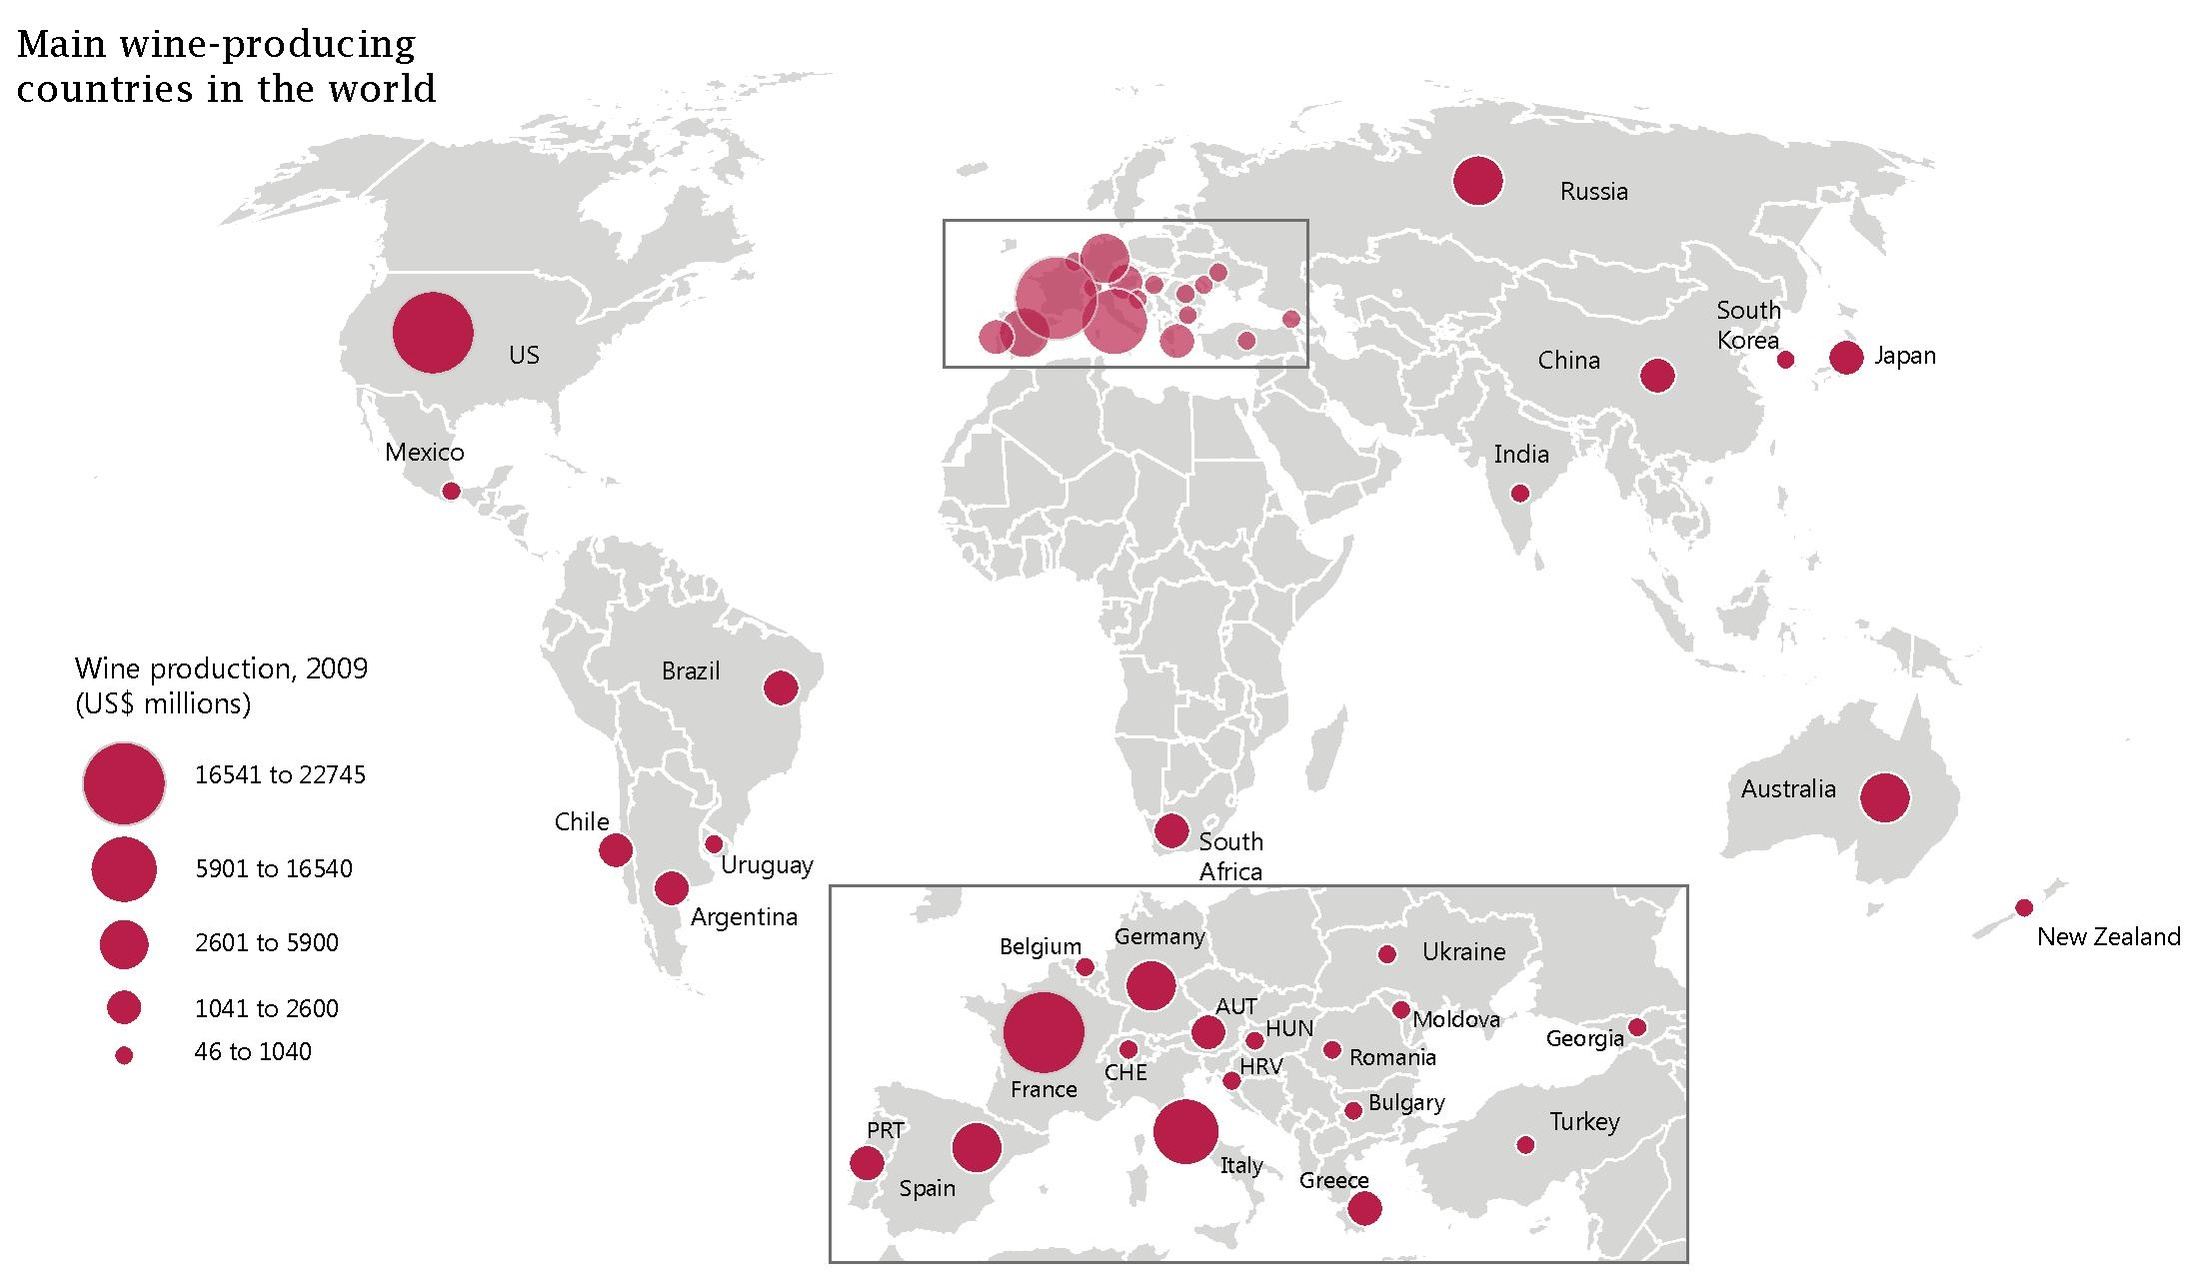
\includegraphics[width=0.8\columnwidth]{../assets/winerieswikipedia.jpg}
\caption{Map from Wikipedia with most relevant wine regions. Note the difference between the figure generated from our dataset (Figure 1) and this map.}
\end{figure}
Apart from the representativeness of our dataset, we consider the amount
of information present, or the usefulness of our data. Most of the
information we have is categorical, so we will have to generate some
quantitative information to open up the number of possible analyzes or
visualizations that are possible with our data.

\chapter{Exploratory Data Analysis}\label{rmd-basics}
\begin{Shaded}
\begin{Highlighting}[]
\KeywordTok{library}\NormalTok{(tidyverse)}
\KeywordTok{library}\NormalTok{(GGally)}
\end{Highlighting}
\end{Shaded}
\section{Countries}\label{countries}

It will be important to understand the countries that are represented in
our dataset in order to be able to know what types of mapping
capabilities we have to have to create a good experience.
\begin{Shaded}
\begin{Highlighting}[]
\NormalTok{path <-}\StringTok{ "../data/winemag-data-130k-v2.csv"}
\NormalTok{Wine <-}\StringTok{ }\KeywordTok{read_csv}\NormalTok{(path,}
                 \DataTypeTok{col_types =} \KeywordTok{cols}\NormalTok{(}
                     \DataTypeTok{X1 =} \KeywordTok{col_double}\NormalTok{(),}
                     \DataTypeTok{country =} \KeywordTok{col_character}\NormalTok{(),}
                     \DataTypeTok{description =} \KeywordTok{col_character}\NormalTok{(),}
                     \DataTypeTok{designation =} \KeywordTok{col_character}\NormalTok{(),}
                     \DataTypeTok{points =} \KeywordTok{col_double}\NormalTok{(),}
                     \DataTypeTok{price =} \KeywordTok{col_double}\NormalTok{(),}
                     \DataTypeTok{province =} \KeywordTok{col_character}\NormalTok{(),}
                     \DataTypeTok{region_1 =} \KeywordTok{col_character}\NormalTok{(),}
                     \DataTypeTok{region_2 =} \KeywordTok{col_character}\NormalTok{(),}
                     \DataTypeTok{taster_name =} \KeywordTok{col_character}\NormalTok{(),}
                     \DataTypeTok{taster_twitter_handle =} \KeywordTok{col_character}\NormalTok{(),}
                     \DataTypeTok{title =} \KeywordTok{col_character}\NormalTok{(),}
                     \DataTypeTok{variety =} \KeywordTok{col_character}\NormalTok{(),}
                     \DataTypeTok{winery =} \KeywordTok{col_character}\NormalTok{()),}
                 \DataTypeTok{progress =} \OtherTok{FALSE}
\NormalTok{                 ) }\OperatorTok
\StringTok{    }\KeywordTok{rename}\NormalTok{(}\DataTypeTok{id =}\NormalTok{ X1)}
\end{Highlighting}
\end{Shaded}
\begin{Shaded}
\begin{Highlighting}[]
\NormalTok{top_countries_tbl <-}\StringTok{ }\NormalTok{Wine }\OperatorTok
\StringTok{    }\KeywordTok{mutate}\NormalTok{(}\DataTypeTok{country =} \KeywordTok{fct_explicit_na}\NormalTok{(country)) }\OperatorTok
\StringTok{    }\KeywordTok{mutate}\NormalTok{(}\DataTypeTok{country =} \KeywordTok{fct_lump}\NormalTok{(country, }\DecValTok{12}\NormalTok{)) }\OperatorTok
\StringTok{    }\KeywordTok{count}\NormalTok{(country, }\DataTypeTok{sort =} \OtherTok{TRUE}\NormalTok{) }\OperatorTok
\StringTok{    }\KeywordTok{mutate}\NormalTok{(}\DataTypeTok{prop =}\NormalTok{ n }\OperatorTok{/}\StringTok{ }\KeywordTok{sum}\NormalTok{(n))}

\NormalTok{top_countries_tbl}
\end{Highlighting}
\end{Shaded}
\begin{verbatim}
     # A tibble: 13 x 3
        country          n   prop
        <fct>        <int>  <dbl>
      1 US           54504 0.419 
      2 France       22093 0.170 
      3 Italy        19540 0.150 
      4 Spain         6645 0.0511
      5 Portugal      5691 0.0438
      6 Chile         4472 0.0344
      7 Argentina     3800 0.0292
      8 Austria       3345 0.0257
      9 Other         2567 0.0198
     10 Australia     2329 0.0179
     11 Germany       2165 0.0167
     12 New Zealand   1419 0.0109
     13 South Africa  1401 0.0108
\end{verbatim}
The top 13 categories, including the lumped-together category of
``Other'' consist of those categories which have a count consisting of
more than 1\% of the observations in the dataset.

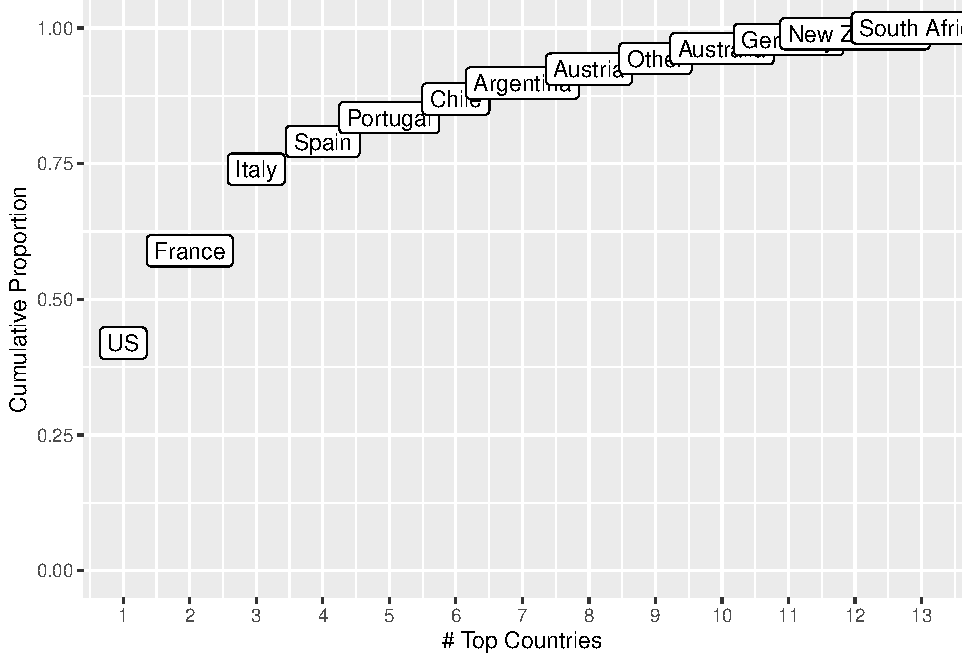
\includegraphics{thesis_files/figure-latex/countries2-1.pdf}

Note that most of the observations, in fact, more than 90\% of the
observations are contained in the 8 most represented countries and 80\%
on the top 4, and 60\% on the top 2 (USA and France).

It looks like it will be possible to create an interactive map. Now we
need to geolocate the wineries. Worst case scenario we have the
countries and their representation in the dataset.

Another interesting fact is that since 40\% of the observations come
from the USA, then perhaps it will be possible to get historical
information to add quantitative predictors to our dataset, but it is not
crucial since our focus is in the presentation of the data.

\section{Wineries}\label{wineries}

Is there a similar concentration for the wineries? Turns out no. Lumping
won't work because there are just so many wineries and there aren't any
ones that particularly dominate.
\begin{Shaded}
\begin{Highlighting}[]
\NormalTok{top_wineries_tbl <-}\StringTok{ }\NormalTok{Wine }\OperatorTok
\StringTok{    }\KeywordTok{count}\NormalTok{(winery, }\DataTypeTok{sort =} \OtherTok{TRUE}\NormalTok{) }\OperatorTok
\StringTok{    }\KeywordTok{mutate}\NormalTok{(}\DataTypeTok{prop =}\NormalTok{ n }\OperatorTok{/}\StringTok{ }\KeywordTok{sum}\NormalTok{(n)) }\OperatorTok
\StringTok{    }\KeywordTok{mutate}\NormalTok{(}\DataTypeTok{prop_cumulative =} \KeywordTok{cumsum}\NormalTok{(prop)) }

\NormalTok{mean_prop <-}\StringTok{ }\KeywordTok{mean}\NormalTok{(top_wineries_tbl}\OperatorTok{$}\NormalTok{prop)}
\NormalTok{mean_prop}
\end{Highlighting}
\end{Shaded}
\begin{verbatim}
     [1] 5.967655e-05
\end{verbatim}
\begin{Shaded}
\begin{Highlighting}[]
\NormalTok{top_wineries_tbl }\OperatorTok
\StringTok{    }\KeywordTok{ggplot}\NormalTok{(}\KeywordTok{aes}\NormalTok{(}\DataTypeTok{x =}\NormalTok{ prop)) }\OperatorTok{+}
\StringTok{    }\KeywordTok{geom_histogram}\NormalTok{(}\DataTypeTok{bins =} \DecValTok{30}\NormalTok{) }\OperatorTok{+}
\StringTok{    }\KeywordTok{geom_vline}\NormalTok{(}\DataTypeTok{xintercept =}\NormalTok{ mean_prop, }\DataTypeTok{color =} \StringTok{"red"}\NormalTok{)}
\end{Highlighting}
\end{Shaded}
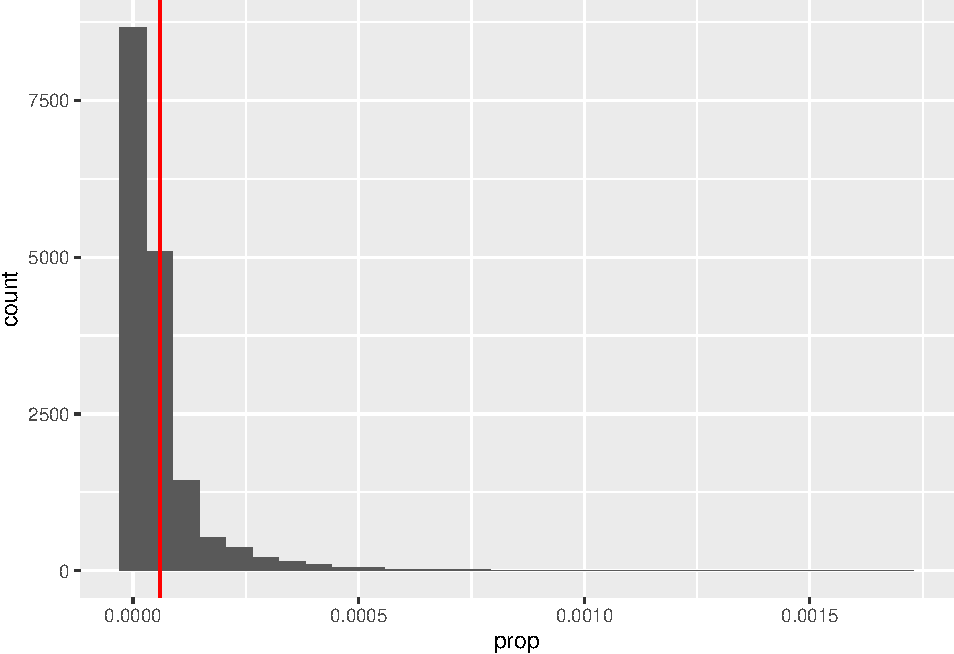
\includegraphics{thesis_files/figure-latex/wineries1-1.pdf}

The table below summarizes the information for the proportions of each
winery.
\begin{Shaded}
\begin{Highlighting}[]
\KeywordTok{summary}\NormalTok{(top_wineries_tbl)}
\end{Highlighting}
\end{Shaded}
\begin{verbatim}
         winery                n                prop          
      Length:16757       Min.   :  1.000   Min.   :7.694e-06  
      Class :character   1st Qu.:  1.000   1st Qu.:7.694e-06  
      Mode  :character   Median :  3.000   Median :2.308e-05  
                         Mean   :  7.756   Mean   :5.968e-05  
                         3rd Qu.:  8.000   3rd Qu.:6.155e-05  
                         Max.   :222.000   Max.   :1.708e-03  
      prop_cumulative   
      Min.   :0.001708  
      1st Qu.:0.721630  
      Median :0.892214  
      Mean   :0.807783  
      3rd Qu.:0.967770  
      Max.   :1.000000
\end{verbatim}
From the summary we note that half of the wineries contain more than
90\% of the observations, and 25\% of the wineries contain more than
70\% of the observations. However there are 16757 wineries which means
that 25\% of the observations is around 4000 wineries.

If we need to geolocate the wineries and we run into trouble, then
perhaps only doing half will suffice for our visualization.

\section{Variety}\label{variety}

Variety of a wine refers to the type of grape that is used - for
example, among white grape wines, there are varieties such as Sauvignon
Blanc, Chardonnay, and Riesling. Among red grape wines, some varieties
include Merlot, Cabernet Sauvignon, and Pinot Noir.
\begin{Shaded}
\begin{Highlighting}[]
\NormalTok{top_varieties_tbl <-}\StringTok{ }\NormalTok{Wine }\OperatorTok
\StringTok{    }\KeywordTok{count}\NormalTok{(variety, }\DataTypeTok{sort =} \OtherTok{TRUE}\NormalTok{) }\OperatorTok
\StringTok{    }\KeywordTok{mutate}\NormalTok{(}\DataTypeTok{prop =}\NormalTok{ n }\OperatorTok{/}\StringTok{ }\KeywordTok{sum}\NormalTok{(n)) }\OperatorTok
\StringTok{    }\KeywordTok{mutate}\NormalTok{(}\DataTypeTok{prop_cumulative =} \KeywordTok{cumsum}\NormalTok{(prop)) }

\KeywordTok{summary}\NormalTok{(top_varieties_tbl)}
\end{Highlighting}
\end{Shaded}
\begin{verbatim}
        variety                n                 prop          
      Length:708         Min.   :    1.00   Min.   :7.690e-06  
      Class :character   1st Qu.:    2.00   1st Qu.:1.539e-05  
      Mode  :character   Median :    6.00   Median :4.616e-05  
                         Mean   :  183.57   Mean   :1.412e-03  
                         3rd Qu.:   28.25   3rd Qu.:2.174e-04  
                         Max.   :13272.00   Max.   :1.021e-01  
      prop_cumulative 
      Min.   :0.1021  
      1st Qu.:0.9749  
      Median :0.9937  
      Mean   :0.9654  
      3rd Qu.:0.9984  
      Max.   :1.0000
\end{verbatim}
\begin{Shaded}
\begin{Highlighting}[]
\NormalTok{top_varieties_tbl }\OperatorTok
\StringTok{  }\KeywordTok{arrange}\NormalTok{(}\KeywordTok{desc}\NormalTok{(prop)) }\OperatorTok
\StringTok{  }\KeywordTok{head}\NormalTok{()}
\end{Highlighting}
\end{Shaded}
\begin{verbatim}
     # A tibble: 6 x 4
       variety                      n   prop prop_cumulative
       <chr>                    <int>  <dbl>           <dbl>
     1 Pinot Noir               13272 0.102            0.102
     2 Chardonnay               11753 0.0904           0.193
     3 Cabernet Sauvignon        9472 0.0729           0.265
     4 Red Blend                 8946 0.0688           0.334
     5 Bordeaux-style Red Blend  6915 0.0532           0.387
     6 Riesling                  5189 0.0399           0.427
\end{verbatim}
We can see from the summary that with among wine variety, 25\% of the
varieties include more than 97\% of of the wines and half of the
varieties account for more than 99\% of the observed wines.
Additionally, Pinot Noir accounts for more than 10\% of the wines,
followed by Chardonnay with 9.0\%, Cabernet Sauvignon with 7.3\%, and
Red Blend with 6.9\%.

\section{Designation}\label{designation}

Designation is a tricky variable to work with. It refers to a label
placed on the wine by the winemaker in regulation with rules of the
country, although not every country has the same rules. For example, the
designation of ``Reserve'' wine generally means the wine has been set
aside to age for a longer time than other wines generally would, and it
often implies a higher quality. While ``Reserva'' refers to reserve
wines in Spain, and ``Riserva'' to those in Italy, the two countries
have different rules about how long the wine must be aged for in order
to receive their respective designations. Other countries, like the
U.S., don't have any rules in general. Given this general lack of
universality of designation, this variable likely will not mean much in
our project, but we can still look at its characteristics.
\begin{Shaded}
\begin{Highlighting}[]
\NormalTok{top_designation_tbl <-}\StringTok{ }\NormalTok{Wine }\OperatorTok
\StringTok{    }\KeywordTok{count}\NormalTok{(designation, }\DataTypeTok{sort =} \OtherTok{TRUE}\NormalTok{) }\OperatorTok
\StringTok{    }\KeywordTok{mutate}\NormalTok{(}\DataTypeTok{prop =}\NormalTok{ n }\OperatorTok{/}\StringTok{ }\KeywordTok{sum}\NormalTok{(n)) }\OperatorTok
\StringTok{    }\KeywordTok{mutate}\NormalTok{(}\DataTypeTok{prop_cumulative =} \KeywordTok{cumsum}\NormalTok{(prop)) }

\KeywordTok{summary}\NormalTok{(top_designation_tbl)}
\end{Highlighting}
\end{Shaded}
\begin{verbatim}
      designation              n                 prop          
      Length:37980       Min.   :    1.00   Min.   :7.690e-06  
      Class :character   1st Qu.:    1.00   1st Qu.:7.690e-06  
      Mode  :character   Median :    1.00   Median :7.690e-06  
                         Mean   :    3.42   Mean   :2.633e-05  
                         3rd Qu.:    2.00   3rd Qu.:1.539e-05  
                         Max.   :37465.00   Max.   :2.883e-01  
      prop_cumulative 
      Min.   :0.2883  
      1st Qu.:0.7374  
      Median :0.8539  
      Mean   :0.8205  
      3rd Qu.:0.9269  
      Max.   :1.0000
\end{verbatim}
\begin{Shaded}
\begin{Highlighting}[]
\NormalTok{top_designation_tbl }\OperatorTok
\StringTok{  }\KeywordTok{arrange}\NormalTok{(}\KeywordTok{desc}\NormalTok{(prop)) }\OperatorTok
\StringTok{  }\KeywordTok{head}\NormalTok{()}
\end{Highlighting}
\end{Shaded}
\begin{verbatim}
     # A tibble: 6 x 4
       designation      n    prop prop_cumulative
       <chr>        <int>   <dbl>           <dbl>
     1 <NA>         37465 0.288             0.288
     2 Reserve       2009 0.0155            0.304
     3 Estate        1322 0.0102            0.314
     4 Reserva       1259 0.00969           0.324
     5 Riserva        698 0.00537           0.329
     6 Estate Grown   621 0.00478           0.334
\end{verbatim}
While 28.8\% of the wines do not have a designation, 25\% of the
designations contain more than 73\% of the wines. We see that of the
most common 5 designations, three of them are related to reserve wines
but in different languages, while the other two refer to estate wines -
wines in which the grapes are grown and the wine is made in the same
location.

\section{Taster}\label{taster}

The tasters are Wine Enthusiast Magazine wine reviewers.
\begin{Shaded}
\begin{Highlighting}[]
\NormalTok{top_taster_tbl <-}\StringTok{ }\NormalTok{Wine }\OperatorTok
\StringTok{    }\KeywordTok{mutate}\NormalTok{(}\DataTypeTok{taster_name =} \KeywordTok{fct_explicit_na}\NormalTok{(taster_name)) }\OperatorTok
\StringTok{    }\KeywordTok{mutate}\NormalTok{(}\DataTypeTok{taster_name =} \KeywordTok{fct_lump}\NormalTok{(taster_name, }\DecValTok{15}\NormalTok{)) }\OperatorTok
\StringTok{    }\KeywordTok{count}\NormalTok{(taster_name, }\DataTypeTok{sort =} \OtherTok{TRUE}\NormalTok{) }\OperatorTok
\StringTok{    }\KeywordTok{mutate}\NormalTok{(}\DataTypeTok{prop =}\NormalTok{ n }\OperatorTok{/}\StringTok{ }\KeywordTok{sum}\NormalTok{(n))}

\NormalTok{top_taster_tbl}
\end{Highlighting}
\end{Shaded}
\begin{verbatim}
     # A tibble: 16 x 3
        taster_name            n    prop
        <fct>              <int>   <dbl>
      1 (Missing)          26244 0.202  
      2 Roger Voss         25514 0.196  
      3 Michael Schachner  15134 0.116  
      4 Kerin O’Keefe      10776 0.0829 
      5 Virginie Boone      9537 0.0734 
      6 Paul Gregutt        9532 0.0733 
      7 Matt Kettmann       6332 0.0487 
      8 Joe Czerwinski      5147 0.0396 
      9 Sean P. Sullivan    4966 0.0382 
     10 Anna Lee C. Iijima  4415 0.0340 
     11 Jim Gordon          4177 0.0321 
     12 Anne Krebiehl MW    3685 0.0284 
     13 Lauren Buzzeo       1835 0.0141 
     14 Susan Kostrzewa     1085 0.00835
     15 Other               1078 0.00829
     16 Mike DeSimone        514 0.00395
\end{verbatim}
While 20\% of the wines do not have tasters listed, 19.6\% of the wines
were tasted by Roger Voss, followed by 11.6\% which were tasted by
Michael Schachner. A potentially interesting side project could be to
try and differentiate the wine descriptions between tasters, or to
search for patterns in each taster's preferred wines.

We can speculate if any of the tasters are biased for more positive or
negative reviews by looking at mean points per taster:
\begin{Shaded}
\begin{Highlighting}[]
\NormalTok{Wine }\OperatorTok
\StringTok{  }\KeywordTok{group_by}\NormalTok{(taster_name) }\OperatorTok
\StringTok{  }\KeywordTok{summarize}\NormalTok{(}\DataTypeTok{meanpoints =} \KeywordTok{mean}\NormalTok{(points)) }\OperatorTok
\StringTok{  }\KeywordTok{arrange}\NormalTok{(}\KeywordTok{desc}\NormalTok{(meanpoints))}
\end{Highlighting}
\end{Shaded}
\begin{verbatim}
     # A tibble: 20 x 2
        taster_name        meanpoints
        <chr>                   <dbl>
      1 Anne Krebiehl MW         90.6
      2 Matt Kettmann            90.0
      3 Virginie Boone           89.2
      4 Mike DeSimone            89.1
      5 Paul Gregutt             89.1
      6 Kerin O’Keefe            88.9
      7 Sean P. Sullivan         88.8
      8 Roger Voss               88.7
      9 Jim Gordon               88.6
     10 Joe Czerwinski           88.5
     11 Anna Lee C. Iijima       88.4
     12 Jeff Jenssen             88.3
     13 Christina Pickard        87.8
     14 <NA>                     87.8
     15 Lauren Buzzeo            87.7
     16 Michael Schachner        86.9
     17 Fiona Adams              86.9
     18 Susan Kostrzewa          86.6
     19 Carrie Dykes             86.4
     20 Alexander Peartree       85.9
\end{verbatim}
The mean points per taster range between 85.9 and 90.6. Although there
are likely many factors underlying these differences in points between
reviewers, if I were a wine maker, I would want Anne Krebiehl MW or Matt
Kettmann reviewing my wine, not Alexander Peartree.

\section{Points}\label{points}

Points is the variable we will be trying to predict.
\begin{Shaded}
\begin{Highlighting}[]
\NormalTok{points_tbl <-}\StringTok{ }\NormalTok{Wine }\OperatorTok
\StringTok{    }\KeywordTok{count}\NormalTok{(points, }\DataTypeTok{sort =} \OtherTok{TRUE}\NormalTok{) }\OperatorTok
\StringTok{    }\KeywordTok{mutate}\NormalTok{(}\DataTypeTok{prop =}\NormalTok{ n }\OperatorTok{/}\StringTok{ }\KeywordTok{sum}\NormalTok{(n))}

\KeywordTok{summary}\NormalTok{(points_tbl)}
\end{Highlighting}
\end{Shaded}
\begin{verbatim}
          points          n              prop          
      Min.   : 80   Min.   :   19   Min.   :0.0001462  
      1st Qu.: 85   1st Qu.:  523   1st Qu.:0.0040240  
      Median : 90   Median : 3758   Median :0.0289141  
      Mean   : 90   Mean   : 6189   Mean   :0.0476191  
      3rd Qu.: 95   3rd Qu.:11359   3rd Qu.:0.0873964  
      Max.   :100   Max.   :17207   Max.   :0.1323911
\end{verbatim}
\begin{Shaded}
\begin{Highlighting}[]
\NormalTok{points_tbl }\OperatorTok
\StringTok{  }\KeywordTok{ggplot}\NormalTok{(}\KeywordTok{aes}\NormalTok{(}\DataTypeTok{x =}\NormalTok{ points, }\DataTypeTok{y =}\NormalTok{ prop)) }\OperatorTok{+}
\StringTok{  }\KeywordTok{geom_bar}\NormalTok{(}\DataTypeTok{stat =} \StringTok{"identity"}\NormalTok{)}
\end{Highlighting}
\end{Shaded}
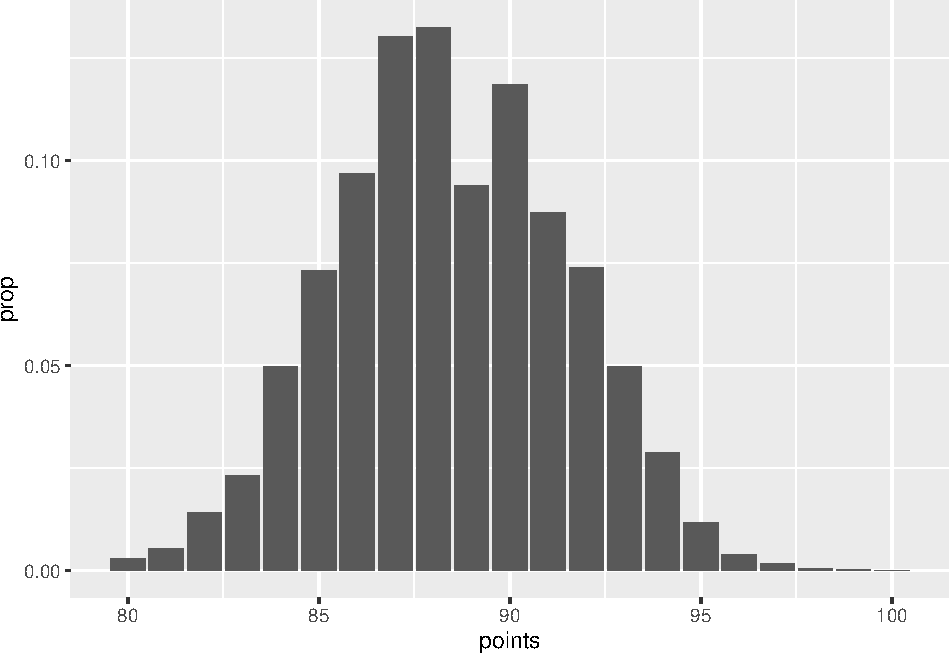
\includegraphics{thesis_files/figure-latex/points-1.pdf}

The points look fairly normally distributed - there might be a slight
right skew due to very few wines being rated over 95 points. The points
range from 80-100 with both mean and median of 90 points.

\section{Price}\label{price}
\begin{Shaded}
\begin{Highlighting}[]
\NormalTok{price_tbl <-}\StringTok{ }\NormalTok{Wine }\OperatorTok
\StringTok{    }\KeywordTok{count}\NormalTok{(price, }\DataTypeTok{sort =} \OtherTok{TRUE}\NormalTok{) }\OperatorTok
\StringTok{    }\KeywordTok{mutate}\NormalTok{(}\DataTypeTok{prop =}\NormalTok{ n }\OperatorTok{/}\StringTok{ }\KeywordTok{sum}\NormalTok{(n)) }\OperatorTok
\StringTok{    }\KeywordTok{mutate}\NormalTok{(}\DataTypeTok{prop_cumulative =} \KeywordTok{cumsum}\NormalTok{(prop)) }

\KeywordTok{summary}\NormalTok{(price_tbl)}
\end{Highlighting}
\end{Shaded}
\begin{verbatim}
          price              n               prop           prop_cumulative  
      Min.   :   4.0   Min.   :   1.0   Min.   :7.690e-06   Min.   :0.06922  
      1st Qu.: 101.2   1st Qu.:   1.0   1st Qu.:7.690e-06   1st Qu.:0.98640  
      Median : 203.5   Median :   4.0   Median :3.078e-05   Median :0.99761  
      Mean   : 293.9   Mean   : 332.4   Mean   :2.558e-03   Mean   :0.95011  
      3rd Qu.: 369.8   3rd Qu.:  47.0   3rd Qu.:3.616e-04   3rd Qu.:0.99925  
      Max.   :3300.0   Max.   :8996.0   Max.   :6.922e-02   Max.   :1.00000  
      NA's   :1
\end{verbatim}
We can see from the table that the price for wine ranges between 4 and
3,300 USD. More than 98\% of the wines are under 101.20 USD, and more
than 99.7\% of the wines are less than 203.5 USD.

\section{Description}\label{description}

Here is an example of the description.
\begin{Shaded}
\begin{Highlighting}[]
\NormalTok{Wine }\OperatorTok\StringTok{ }\KeywordTok{pull}\NormalTok{(description) }\OperatorTok\StringTok{ }\KeywordTok{pluck}\NormalTok{(}\DecValTok{1}\NormalTok{)}
\end{Highlighting}
\end{Shaded}
{[}1{]} ``Aromas include tropical fruit, broom, brimstone and dried
herb. The palate isn't overly expressive, offering unripened apple,
citrus and dried sage alongside brisk acidity.''

This is one example. We will want to extract features from the
description in order to incorporate this information into any model we
do.

\section{Province and Regions}\label{province-and-regions}

Province and regions are related to country for self-explanatory
reasons. Region is a smaller area of a province. Let's just explore
province.
\begin{Shaded}
\begin{Highlighting}[]
\NormalTok{top_province_tbl <-}\StringTok{ }\NormalTok{Wine }\OperatorTok
\StringTok{    }\KeywordTok{count}\NormalTok{(province, }\DataTypeTok{sort =} \OtherTok{TRUE}\NormalTok{) }\OperatorTok
\StringTok{    }\KeywordTok{mutate}\NormalTok{(}\DataTypeTok{prop =}\NormalTok{ n }\OperatorTok{/}\StringTok{ }\KeywordTok{sum}\NormalTok{(n)) }\OperatorTok
\StringTok{    }\KeywordTok{mutate}\NormalTok{(}\DataTypeTok{prop_cumulative =} \KeywordTok{cumsum}\NormalTok{(prop)) }

\KeywordTok{summary}\NormalTok{(top_province_tbl)}
\end{Highlighting}
\end{Shaded}
\begin{verbatim}
        province               n                 prop          
      Length:426         Min.   :    1.00   Min.   :7.690e-06  
      Class :character   1st Qu.:    3.00   1st Qu.:2.308e-05  
      Mode  :character   Median :   12.00   Median :9.233e-05  
                         Mean   :  305.10   Mean   :2.347e-03  
                         3rd Qu.:   53.75   3rd Qu.:4.135e-04  
                         Max.   :36247.00   Max.   :2.789e-01  
      prop_cumulative 
      Min.   :0.2789  
      1st Qu.:0.9733  
      Median :0.9935  
      Mean   :0.9593  
      3rd Qu.:0.9987  
      Max.   :1.0000
\end{verbatim}
\begin{Shaded}
\begin{Highlighting}[]
\NormalTok{top_province_tbl }\OperatorTok
\StringTok{  }\KeywordTok{arrange}\NormalTok{(}\KeywordTok{desc}\NormalTok{(prop)) }\OperatorTok
\StringTok{  }\KeywordTok{head}\NormalTok{()}
\end{Highlighting}
\end{Shaded}
\begin{verbatim}
     # A tibble: 6 x 4
       province       n   prop prop_cumulative
       <chr>      <int>  <dbl>           <dbl>
     1 California 36247 0.279            0.279
     2 Washington  8639 0.0665           0.345
     3 Bordeaux    5941 0.0457           0.391
     4 Tuscany     5897 0.0454           0.436
     5 Oregon      5373 0.0413           0.478
     6 Burgundy    3980 0.0306           0.508
\end{verbatim}
Unsurprisingly, provinces in the U.S., France, and Italy dominate the
top provinces list. A whopping 28\% of our wines come from California
alone.

\chapter{Text Analysis and Prediction}\label{math-sci}

\section{Extracting Features from
Text}\label{extracting-features-from-text}

A key part of this project is learning how to extract features from
text. In the case of our data with wine reviews, the largest body of
text we have is from the description variable. First we'll load in our
data.

First, we can look at some exploratory plots. For example, following
\href{https://www.kaggle.com/nnnnick/predicting-wine-ratings-using-lightgbm-text2vec}{code
from Kaggle user nnnnick (2018)}\footnote{(``Predicting wine ratings
  using lightgbm + text2vec,'' 2018)}, we can look at the words in the
wine description with the highest and lowest mean scores:

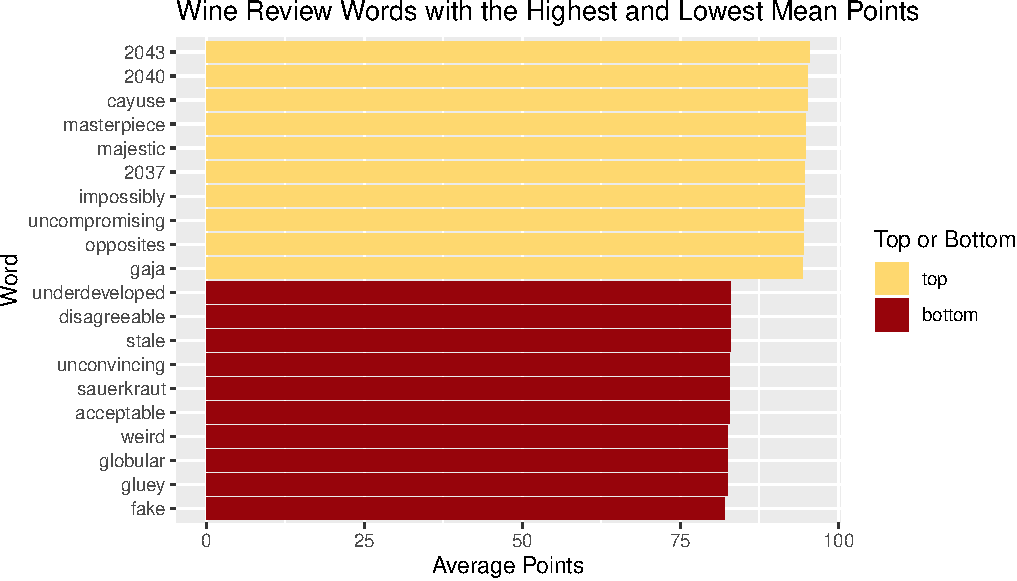
\includegraphics{thesis_files/figure-latex/figpoints-1.pdf}

For the words with the top mean points, we can see several words that
are actually years in the future - for example, 2043 and 2040. This is
because many wine reviews of good wines will included something like
``This wine will age well to 2040'' or something of the sort. Some words
in the top 10 with the highest mean point values may not be familiar to
most people. ``Cayuse,'' for example, is the name of vineyards in
Washington state that are famous for tasty wines. Simialrly, ``Gaja'' is
the name of a famous Italian producer of wine.

Looking at the words with the lowest mean points, nobody wants to drink
a wine that's described as ``gluey'' or ``fake.'' How often do these
words show up though, and how can we use them in a predictive model? To
find out, we need to create a document-term matrix, which shows the the
frequency of terms that occur in a collection of documents.

\subsection{Creating a Document-Term Matrix
(DTM)}\label{creating-a-document-term-matrix-dtm}

A DTM is a matrix in which the rows correspond to documents in a corpus
(in our case, each wine description constitutes a document) and each
column corresponds to terms, or words. This code to create a DTM for our
wine dataset is based on
\href{https://datawarrior.wordpress.com/2018/01/22/document-term-matrix-text-mining-in-r-and-python/}{this
blog post}\footnote{Ho (2018)}.
\begin{Shaded}
\begin{Highlighting}[]
\CommentTok{#Create DTM}
\NormalTok{dtm <-}\StringTok{ }\KeywordTok{CreateDtm}\NormalTok{(Wine}\OperatorTok{$}\NormalTok{description,}
                \DataTypeTok{doc_names =}\NormalTok{ Wine}\OperatorTok{$}\NormalTok{id,}
                \DataTypeTok{ngram_window =} \KeywordTok{c}\NormalTok{(}\DecValTok{1}\NormalTok{, }\DecValTok{1}\NormalTok{),}
                \DataTypeTok{lower =} \OtherTok{TRUE}\NormalTok{,}
                \DataTypeTok{remove_punctuation =} \OtherTok{TRUE}\NormalTok{,}
                \DataTypeTok{remove_numbers =} \OtherTok{TRUE}\NormalTok{,}
                \DataTypeTok{stem_lemma_function =}\NormalTok{ wordStem)}
\end{Highlighting}
\end{Shaded}
The resulting DTM is huge - about 43 megabytes with close to 3 billion
elements. We need to create some functions that will allow us to use the
DTM:
\begin{Shaded}
\begin{Highlighting}[]
\CommentTok{#Create functions}
\NormalTok{get.token.occurrences<-}\StringTok{ }\ControlFlowTok{function}\NormalTok{(dtm, token)}
\NormalTok{  dtm[, token] }\OperatorTok\StringTok{ }\KeywordTok{as.data.frame}\NormalTok{() }\OperatorTok\StringTok{ }\KeywordTok{rename}\NormalTok{(}\DataTypeTok{count=}\StringTok{"."}\NormalTok{) }\OperatorTok
\StringTok{  }\KeywordTok{mutate}\NormalTok{(}\DataTypeTok{token=}\KeywordTok{row.names}\NormalTok{(.)) }\OperatorTok\StringTok{ }\KeywordTok{arrange}\NormalTok{(}\OperatorTok{-}\NormalTok{count)}
 
\NormalTok{get.total.freq<-}\StringTok{ }\ControlFlowTok{function}\NormalTok{(dtm, token) dtm[, token] }\OperatorTok\StringTok{ }\NormalTok{sum}
 
\NormalTok{get.doc.freq<-}\StringTok{ }\ControlFlowTok{function}\NormalTok{(dtm, token)}
\NormalTok{  dtm[, token] }\OperatorTok\StringTok{ }\KeywordTok{as.data.frame}\NormalTok{() }\OperatorTok\StringTok{ }\KeywordTok{rename}\NormalTok{(}\DataTypeTok{count=}\StringTok{"."}\NormalTok{) }\OperatorTok
\StringTok{  }\KeywordTok{filter}\NormalTok{(count}\OperatorTok{>}\DecValTok{0}\NormalTok{) }\OperatorTok\StringTok{ }\KeywordTok{pull}\NormalTok{(count) }\OperatorTok\StringTok{ }\NormalTok{length}
\end{Highlighting}
\end{Shaded}
Now we can see how many wines are actually described as ``fake'':
\begin{Shaded}
\begin{Highlighting}[]
\NormalTok{dtm }\OperatorTok\StringTok{ }\KeywordTok{get.doc.freq}\NormalTok{(}\KeywordTok{wordStem}\NormalTok{(}\StringTok{"fake"}\NormalTok{))}
\end{Highlighting}
\end{Shaded}
\begin{verbatim}
     [1] 13
\end{verbatim}
Which 13 wines?
\begin{Shaded}
\begin{Highlighting}[]
\NormalTok{fakewines <-}\StringTok{ }\NormalTok{dtm }\OperatorTok\StringTok{ }\KeywordTok{get.token.occurrences}\NormalTok{(}\KeywordTok{wordStem}\NormalTok{(}\StringTok{"fake"}\NormalTok{)) }\OperatorTok\StringTok{ }\KeywordTok{head}\NormalTok{(}\DecValTok{13}\NormalTok{)}
\NormalTok{Wine}\OperatorTok{$}\NormalTok{title[}\KeywordTok{c}\NormalTok{(}\KeywordTok{as.numeric}\NormalTok{(fakewines}\OperatorTok{$}\NormalTok{token))]}
\end{Highlighting}
\end{Shaded}
\begin{verbatim}
      [1] "Robert Stemmler 2005 Nugent Vineyard Pinot Noir (Russian River Valley)"          
      [2] "Funky Llama 2011 Merlot (Mendoza)"                                               
      [3] "Pierre Chardigny 2015 Vieilles Vignes  (Saint-Véran)"                            
      [4] "Mellisoni 2016 Estate Pinot Grigio (Lake Chelan)"                                
      [5] "Pradorey 2016 Tempranillo-Merlot Fermentado en Barrica Rosado (Ribera del Duero)"
      [6] "Skylite 2005 Skylite Vineyard Merlot (Walla Walla Valley (WA))"                  
      [7] "Black Stallion 2014 Cabernet Sauvignon (Napa Valley)"                            
      [8] "Adega Cooperativa Ponte de Barca 2013 Ela Rosé (Vinho Verde)"                    
      [9] "St. Julian 2013 Reserve Pinot Grigio (Lake Michigan Shore)"                      
     [10] "Cannonball 2010 Cabernet Sauvignon (California)"                                 
     [11] "Finca Patagonia 2015 Expedicion Pinot Noir (Maule Valley)"                       
     [12] "Loken Cellars NV Reserve Lot 14 Rosé (California)"                               
     [13] "St. Andrews Estate 2000 Ceravolo Chardonnay (Adelaide Hills)"
\end{verbatim}
Let's look at the description of the fourth wine:

{[}1{]} ``Scattershot aromas of generic berry and cinnamon smell forced
and fake. This has a tannic scrubbing mouthfeel and artificial flavors
of chocolate and cheap oak. A green note and burn on the finish do
nothing to help this along.''

Yikes. This seems like a bad wine.

From our document-term matrix, we could create a list of the top words
by frequency and use those in our predictive model. However, if we were
basing our top words by term frequency, we would be including words that
are used so often that they probably don't have much meaning. Therefore,
a better way to rank our words would be term frequency-inverse document
frequency, which will be explained in the next section.

\subsection{Term Frequency-Inverse Document
Frequency}\label{term-frequency-inverse-document-frequency}

Term Frequency-Inverse Document Frequency (TF-IDF) is a statistic that
evaluates how important a word is in a document or corpus. It is
calculated through dividing the term frequency of how often a word
appears in a document by its inverse document frequency, which is the
inverse of the proportion of how many documents in a corpus have a
certain term. Therefore, high frequency terms but with little importance
such as ``the'' or ``and'' will have low TF-IDF values, and so TF-IDF
can be used as a weighting measure in ranking.

TF-IDF will be useful in our prediction model becuase we can include the
words with the higest mean TF-IDF values in our model. Let's see what
these words with the highest mean TF-IDF values are. The following code
has been modified from the one of the
\href{https://cran.r-project.org/web/packages/textmineR/vignettes/a_start_here.html}{cran.R
vignettes of the \texttt{textmineR} package}\footnote{Jones (2018)}.
\begin{Shaded}
\begin{Highlighting}[]
\NormalTok{tf_mat <-}\StringTok{ }\KeywordTok{TermDocFreq}\NormalTok{(}\DataTypeTok{dtm =}\NormalTok{ dtm)}
\KeywordTok{head}\NormalTok{(tf_mat[ }\KeywordTok{order}\NormalTok{(tf_mat}\OperatorTok{$}\NormalTok{term_freq, }\DataTypeTok{decreasing =} \OtherTok{TRUE}\NormalTok{) , ], }\DecValTok{10}\NormalTok{)}
\end{Highlighting}
\end{Shaded}
\begin{verbatim}
              term term_freq doc_freq       idf
     wine     wine     83107    66140 0.6755376
     flavor flavor     70968    65697 0.6822581
     fruit   fruit     63935    55692 0.8474748
     aroma   aroma     41052    40492 1.1662069
     finish finish     40466    40083 1.1763590
     acid     acid     39812    38586 1.2144218
     palat   palat     38636    37796 1.2351081
     drink   drink     33970    33244 1.3634370
     cherri cherri     33590    31328 1.4227991
     tannin tannin     32981    31960 1.4028262
\end{verbatim}
\begin{Shaded}
\begin{Highlighting}[]
\NormalTok{tfidf_mat <-}\StringTok{ }\KeywordTok{t}\NormalTok{(dtm[ , tf_mat}\OperatorTok{$}\NormalTok{term ]) }\OperatorTok{*}\StringTok{ }\NormalTok{tf_mat}\OperatorTok{$}\NormalTok{idf }\CommentTok{#calculating TF-IDF}
\NormalTok{tfidf <-}\StringTok{ }\KeywordTok{t}\NormalTok{(tfidf_mat)}
\NormalTok{tfidf_means <-}\StringTok{ }\KeywordTok{colMeans}\NormalTok{(tfidf) }\CommentTok{#calculating mean values}
\NormalTok{tfidf_means <-}\StringTok{ }\KeywordTok{as.data.frame}\NormalTok{(tfidf_means)}
\NormalTok{tfidf_means}\OperatorTok{$}\NormalTok{word <-}\StringTok{ }\KeywordTok{rownames}\NormalTok{(tfidf_means)}
\CommentTok{#top 200 with highest mean TF-IDF values}
\NormalTok{top200 <-}\StringTok{ }\NormalTok{tfidf_means }\OperatorTok\StringTok{ }\KeywordTok{arrange}\NormalTok{(}\KeywordTok{desc}\NormalTok{(tfidf_means)) }\OperatorTok\StringTok{ }\KeywordTok{top_n}\NormalTok{(}\DecValTok{200}\NormalTok{, tfidf_means)}
\end{Highlighting}
\end{Shaded}
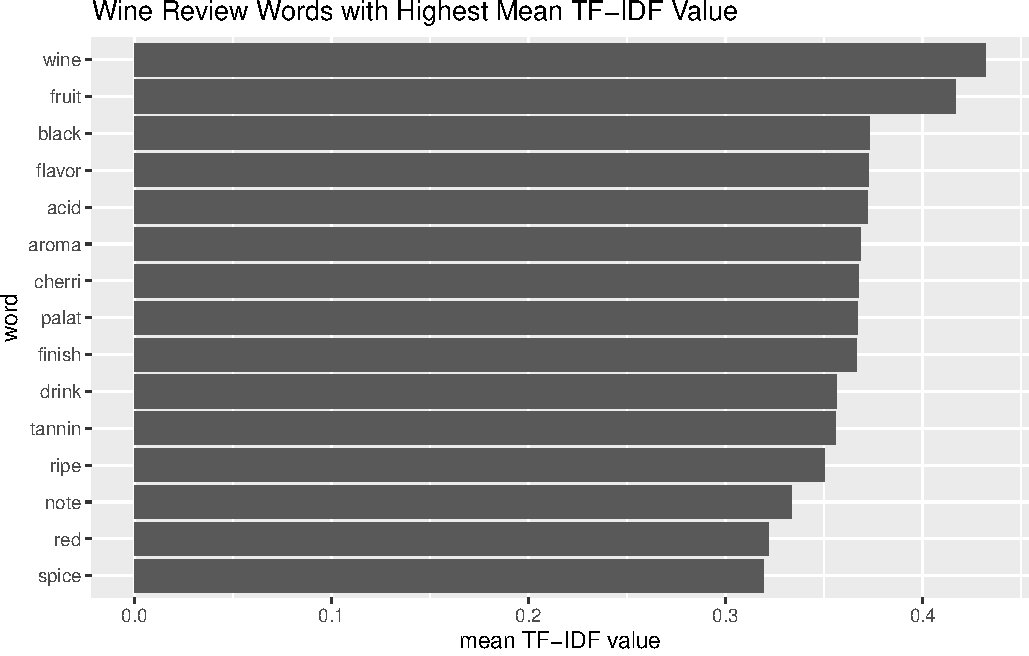
\includegraphics{thesis_files/figure-latex/figtfidf-1.pdf}

``Wine'' and ``fruit'' have especially high mean TF-IDF values, followed
by ``black,'' ``flavor,'' ``acid,'' and ``aroma.''

Now let's see how we can use the DTM in a data frame for prediction.
\begin{Shaded}
\begin{Highlighting}[]
\CommentTok{# Match dtm column names to the words with top 200 mean tf-idf values}
\NormalTok{dtm_small <-}\StringTok{ }\NormalTok{dtm[, }\KeywordTok{colnames}\NormalTok{(dtm) }\OperatorTok\StringTok{ }\NormalTok{top200}\OperatorTok{$}\NormalTok{word]}
\KeywordTok{ncol}\NormalTok{(dtm_small)}
\end{Highlighting}
\end{Shaded}
\begin{verbatim}
     [1] 200
\end{verbatim}
We're left with a document-term matrix with the 200 words with the
highest mean tf-idf value.

\section{Prediction}\label{prediction}

Let's look at predicting wines. We are looking to build a model that can
be implemented for an average user of our web app to input values and
text and receive an output of points.

Because we have a lot of missing data and a mixture of numerical and
categorical data, methods like random forest are difficult to implement.
Let's try gradient boosting, which in R can include categorical
variables of up to 1024 categories (unlike randomForest, which only
allows up to 53 categories per categorical variable).

First, we need to clean our data. We will remove variables that either
1) are factor variables with more than 1024 categories, or 2) are
variables that are not necessarily relevant to an average person looking
to explore wine. An example of variables in the latter category are
\texttt{taster\_name} and \texttt{taster\_twitter\_handle}.
\begin{Shaded}
\begin{Highlighting}[]
\NormalTok{dtm_df <-}\StringTok{ }\KeywordTok{as.data.frame}\NormalTok{(}\KeywordTok{as.matrix}\NormalTok{(dtm_small))}
\NormalTok{dtm_df}\OperatorTok{$}\NormalTok{id <-}\StringTok{ }\KeywordTok{c}\NormalTok{(}\DecValTok{0}\OperatorTok{:}\DecValTok{129970}\NormalTok{)}
\NormalTok{Wine_dtm <-}\StringTok{ }\KeywordTok{left_join}\NormalTok{(Wine, dtm_df, }\DataTypeTok{by =} \StringTok{"id"}\NormalTok{)}
\NormalTok{Wine_dtm <-}\StringTok{ }\NormalTok{Wine_dtm }\OperatorTok
\StringTok{  }\KeywordTok{select}\NormalTok{(}\OperatorTok{-}\NormalTok{id, }\OperatorTok{-}\NormalTok{description, }\OperatorTok{-}\NormalTok{designation, }\OperatorTok{-}\NormalTok{region_}\DecValTok{1}\NormalTok{, }\OperatorTok{-}\NormalTok{region_}\DecValTok{2}\NormalTok{, }\OperatorTok{-}\NormalTok{taster_name,}
         \OperatorTok{-}\NormalTok{taster_twitter_handle, }\OperatorTok{-}\NormalTok{title, }\OperatorTok{-}\NormalTok{winery) }\OperatorTok
\StringTok{  }\KeywordTok{mutate}\NormalTok{(}\DataTypeTok{country =} \KeywordTok{as.factor}\NormalTok{(country),}
         \DataTypeTok{province =} \KeywordTok{as.factor}\NormalTok{(province),}
         \DataTypeTok{variety =} \KeywordTok{as.factor}\NormalTok{(variety))}
\end{Highlighting}
\end{Shaded}
Now we will split our data into training and test sets.
\begin{Shaded}
\begin{Highlighting}[]
\CommentTok{# Test/Train split}
\KeywordTok{set.seed}\NormalTok{(}\DecValTok{1}\NormalTok{)}
\NormalTok{smp_size <-}\StringTok{ }\KeywordTok{floor}\NormalTok{(}\FloatTok{0.8} \OperatorTok{*}\StringTok{ }\KeywordTok{nrow}\NormalTok{(Wine_dtm))}
\NormalTok{train_ind <-}\StringTok{ }\KeywordTok{sample}\NormalTok{(}\KeywordTok{seq_len}\NormalTok{(}\KeywordTok{nrow}\NormalTok{(Wine_dtm)), }\DataTypeTok{size =}\NormalTok{ smp_size)}
\NormalTok{train <-}\StringTok{ }\NormalTok{Wine_dtm[train_ind, ]}
\NormalTok{test <-}\StringTok{ }\NormalTok{Wine_dtm[}\OperatorTok{-}\NormalTok{train_ind, ]}
\end{Highlighting}
\end{Shaded}
Now we can apply a gradient boosting algorithm to create our prediction
model. First, let's try a boosting model with 5 trees. This is not a lot
of trees, so we'd expect that the model wouldn't do so well with
prediction on our test set.
\begin{Shaded}
\begin{Highlighting}[]
\KeywordTok{set.seed}\NormalTok{(}\DecValTok{1}\NormalTok{)}
\NormalTok{boost_wine5 <-}\StringTok{ }\KeywordTok{gbm}\NormalTok{(points }\OperatorTok{~}\StringTok{ }\NormalTok{., }
                   \DataTypeTok{data =}\NormalTok{ train, }
                   \DataTypeTok{distribution =} \StringTok{"gaussian"}\NormalTok{, }
                   \DataTypeTok{n.trees =} \DecValTok{5}\NormalTok{,}
                   \DataTypeTok{interaction.depth =} \DecValTok{4}\NormalTok{)}

\NormalTok{boost_estimate5 <-}\StringTok{ }\KeywordTok{predict}\NormalTok{(boost_wine5, }\CommentTok{# predict on test set }
                         \DataTypeTok{newdata =}\NormalTok{ test,}
                         \DataTypeTok{n.trees =} \DecValTok{5}\NormalTok{,}
                         \DataTypeTok{na.action =} \OtherTok{NULL}\NormalTok{)}
\NormalTok{mse_boost5 <-}\StringTok{ }\KeywordTok{mean}\NormalTok{((boost_estimate5 }\OperatorTok{-}\StringTok{ }\NormalTok{test}\OperatorTok{$}\NormalTok{points)}\OperatorTok{^}\DecValTok{2}\NormalTok{)}
\NormalTok{sqrt_mse5 <-}\StringTok{ }\KeywordTok{sqrt}\NormalTok{(mse_boost5); sqrt_mse5 }\CommentTok{# calculate MSE}
\end{Highlighting}
\end{Shaded}
\begin{verbatim}
     [1] 2.659352
\end{verbatim}
With this model, the prediction is off by an average of 2.6593525
points. That's not great. Let's compare this square root of the MSE to
that of a model where we use 500 trees.
\begin{Shaded}
\begin{Highlighting}[]
\KeywordTok{set.seed}\NormalTok{(}\DecValTok{1}\NormalTok{)}
\NormalTok{boost_wine <-}\StringTok{ }\KeywordTok{gbm}\NormalTok{(points }\OperatorTok{~}\StringTok{ }\NormalTok{., }
                   \DataTypeTok{data =}\NormalTok{ train, }
                   \DataTypeTok{distribution =} \StringTok{"gaussian"}\NormalTok{, }
                   \DataTypeTok{n.trees =} \DecValTok{500}\NormalTok{,}
                   \DataTypeTok{interaction.depth =} \DecValTok{4}\NormalTok{)}

\CommentTok{# Save model to .rds file}
\KeywordTok{saveRDS}\NormalTok{(boost_wine, }\StringTok{"boost_wine500.rds"}\NormalTok{)}
\end{Highlighting}
\end{Shaded}
Running the above chunk takes too long, so we've loaded the model in the
chunk below. We can check to see how well this model with 500 trees does
with prediction on the test set:
\begin{Shaded}
\begin{Highlighting}[]
\CommentTok{# load model}
\NormalTok{boost_wine <-}\StringTok{ }\NormalTok{readr}\OperatorTok{::}\KeywordTok{read_rds}\NormalTok{(}\StringTok{"~/git/Stat495-F19-GroupD/FinalProject/index/data/boost_wine500.rds"}\NormalTok{)}
\NormalTok{boost_estimate <-}\StringTok{ }\KeywordTok{predict}\NormalTok{(boost_wine, }
                         \DataTypeTok{newdata =}\NormalTok{ test, }
                         \DataTypeTok{n.trees =} \DecValTok{500}\NormalTok{,}
                         \DataTypeTok{na.action =} \OtherTok{NULL}\NormalTok{)}
\NormalTok{mse_boost <-}\StringTok{ }\KeywordTok{mean}\NormalTok{((boost_estimate }\OperatorTok{-}\StringTok{ }\NormalTok{test}\OperatorTok{$}\NormalTok{points)}\OperatorTok{^}\DecValTok{2}\NormalTok{)}
\NormalTok{sqrt_mse <-}\StringTok{ }\KeywordTok{sqrt}\NormalTok{(mse_boost); sqrt_mse}
\end{Highlighting}
\end{Shaded}
\begin{verbatim}
     [1] 1.834457
\end{verbatim}
The square root of the mean squared error is 1.834457 - much smaller
than that of the model with only 5 trees. Let's look at the most
important features in this more accurate model.
\begin{Shaded}
\begin{Highlighting}[]
\KeywordTok{top_n}\NormalTok{(}\KeywordTok{summary}\NormalTok{(boost_wine), }\DecValTok{10}\NormalTok{, rel.inf)}
\end{Highlighting}
\end{Shaded}
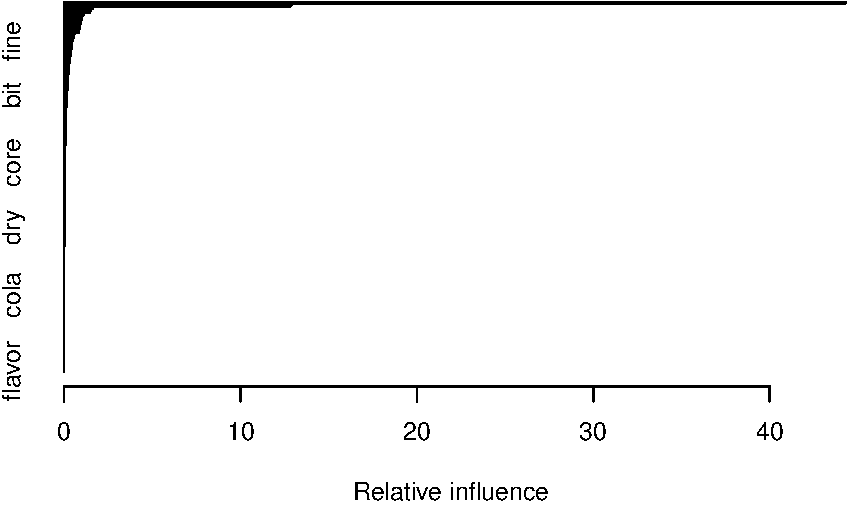
\includegraphics{thesis_files/figure-latex/unnamed-chunk-6-1.pdf}
\begin{verbatim}
             var    rel.inf
     1     price 44.2872441
     2   variety 12.8744278
     3  province 12.8074735
     4      rich  1.6195324
     5   complex  1.5243999
     6     simpl  1.4679213
     7      long  1.1043904
     8    delici  1.0599025
     9     black  0.9946763
     10 concentr  0.9875296
\end{verbatim}
Unsurprisingly, the variable with the most relative influence is price,
followed by variety, then province. Stemmed words that are the most
important are ``rich'', ``complex,'' ``simpl.''

Let's see how this model predicts the points of a wine that is not in
the data set.

For example, we can predict the points of a Portuguese Red Touriga
Nacional wine that is \$35 from Dão with the description: ``This is a
solidly structured wine that has big tannins in place. That will change
as the wine ages further, bringing the rich black fruits forward and
reveling in the perfumed acidity of the wine. Drink from 2021.''

Below, we have created a function called \texttt{estimatepoints} that
uses inputs of country, price, description, province, and variety and
returns a points estimate based on our model.
\begin{Shaded}
\begin{Highlighting}[]
\NormalTok{estimatepoints <-}\StringTok{ }\ControlFlowTok{function}\NormalTok{(country, price, description, province, variety) \{}
\NormalTok{  newwine <-}\StringTok{ }\KeywordTok{data.frame}\NormalTok{(}\DataTypeTok{id =} \DecValTok{1}\NormalTok{, country, price, description, province, }
\NormalTok{                        variety) }\OperatorTok
\StringTok{    }\KeywordTok{mutate}\NormalTok{(}\DataTypeTok{description =} \KeywordTok{as.character}\NormalTok{(description))}
  
  \CommentTok{# Create DTM for new wine}
\NormalTok{  dtm_newwine <-}\StringTok{ }\KeywordTok{CreateDtm}\NormalTok{(newwine}\OperatorTok{$}\NormalTok{description,}
                \DataTypeTok{doc_names =}\NormalTok{ newwine}\OperatorTok{$}\NormalTok{id,}
                \DataTypeTok{ngram_window =} \KeywordTok{c}\NormalTok{(}\DecValTok{1}\NormalTok{, }\DecValTok{1}\NormalTok{),}
                \DataTypeTok{lower =} \OtherTok{TRUE}\NormalTok{,}
                \DataTypeTok{remove_punctuation =} \OtherTok{TRUE}\NormalTok{,}
                \DataTypeTok{remove_numbers =} \OtherTok{TRUE}\NormalTok{,}
                \DataTypeTok{stem_lemma_function =}\NormalTok{ wordStem)}
  \CommentTok{# words in top 200}
\NormalTok{  dtm_newwine2 <-}\StringTok{ }\NormalTok{dtm_newwine[, }\KeywordTok{colnames}\NormalTok{(dtm_newwine) }\OperatorTok\StringTok{ }\NormalTok{top200}\OperatorTok{$}\NormalTok{word]}
\NormalTok{  dtm_newwine_df <-}\StringTok{ }\KeywordTok{as.data.frame}\NormalTok{(}\KeywordTok{as.matrix}\NormalTok{(}\KeywordTok{t}\NormalTok{(dtm_newwine2)))}
  \CommentTok{# find the top 200 words not in new wine but in dtm}
\NormalTok{    otherwords <-}\StringTok{ }\NormalTok{top200 }\OperatorTok
\StringTok{    }\KeywordTok{filter}\NormalTok{(}\OperatorTok{!}\NormalTok{word }\OperatorTok\StringTok{ }\NormalTok{dtm_newwine_df)}
  \CommentTok{# fill the words not in new wine to df with 0}
\NormalTok{  dtm_newwine_df[otherwords}\OperatorTok{$}\NormalTok{word] <-}\StringTok{ }\DecValTok{0}

\NormalTok{  newwine <-}\StringTok{ }\KeywordTok{cbind}\NormalTok{(newwine, dtm_newwine_df) }\CommentTok{# fill in rest of data}
  
  \CommentTok{# Estimate points of new wine}
\NormalTok{  test_estimate <-}\StringTok{ }\KeywordTok{predict}\NormalTok{(boost_wine, }
                         \DataTypeTok{newdata =}\NormalTok{ newwine,}
                         \DataTypeTok{n.trees =} \DecValTok{100}\NormalTok{,}
                         \DataTypeTok{na.action =} \OtherTok{NULL}\NormalTok{)}

  \KeywordTok{return}\NormalTok{(test_estimate)}
\NormalTok{\}}

\CommentTok{# Save function & top200 data frame for use in Shiny app}
\KeywordTok{save}\NormalTok{(top200, estimatepoints, }\DataTypeTok{file=}\StringTok{"estimatepoints_function.Rda"}\NormalTok{)}
\end{Highlighting}
\end{Shaded}
So now to predict the number of points our Portuguese wine would
receive, we can just plug in the input values.
\begin{Shaded}
\begin{Highlighting}[]
\KeywordTok{estimatepoints}\NormalTok{(}\DataTypeTok{country =} \StringTok{"Portugal"}\NormalTok{,}
               \DataTypeTok{price =} \DecValTok{35}\NormalTok{,}
               \DataTypeTok{description =} \StringTok{"This is a solidly structured wine that }
\StringTok{               has big tannins in place. That will change as the wine }
\StringTok{               ages further, bringing the rich black fruits forward }
\StringTok{               and reveling in the perfumed acidity of the wine.}
\StringTok{               Drink from 2021."}\NormalTok{,}
               \DataTypeTok{province =} \StringTok{"Dão"}\NormalTok{,}
               \DataTypeTok{variety =} \StringTok{"Touriga Nacional, Portuguese Red"}\NormalTok{)}
\end{Highlighting}
\end{Shaded}
\begin{verbatim}
     [1] 88.83818
\end{verbatim}
Our model predicts this wine would receive about 89 points. Not bad.

\textbf{Model with just description}

The model we are using to predict points uses variables like price,
province, and variety, which all have much higher relative influence
compared to just the words in the description. What if we removed these
variables with higher relative influence and looked just at how well
words in the description can predict points?

We will select just the points variable and the word variables and set
up a training and test set to create the same gradient boosting model
with just the word variables.
\begin{Shaded}
\begin{Highlighting}[]
\CommentTok{# leaves just the DTM of words}
\NormalTok{Wine_justwords <-}\StringTok{ }\NormalTok{Wine_dtm }\OperatorTok
\StringTok{  }\KeywordTok{select}\NormalTok{(}\OperatorTok{-}\NormalTok{country, }\OperatorTok{-}\NormalTok{price, }\OperatorTok{-}\NormalTok{province, }\OperatorTok{-}\NormalTok{variety) }

\CommentTok{# Train/Test split}
\KeywordTok{set.seed}\NormalTok{(}\DecValTok{1}\NormalTok{)}
\NormalTok{smp_size2 <-}\StringTok{ }\KeywordTok{floor}\NormalTok{(}\FloatTok{0.8} \OperatorTok{*}\StringTok{ }\KeywordTok{nrow}\NormalTok{(Wine_justwords))}
\NormalTok{train_ind2 <-}\StringTok{ }\KeywordTok{sample}\NormalTok{(}\KeywordTok{seq_len}\NormalTok{(}\KeywordTok{nrow}\NormalTok{(Wine_justwords)), }\DataTypeTok{size =}\NormalTok{ smp_size2)}
\NormalTok{train2 <-}\StringTok{ }\NormalTok{Wine_justwords[train_ind2, ]}
\NormalTok{test2 <-}\StringTok{ }\NormalTok{Wine_justwords[}\OperatorTok{-}\NormalTok{train_ind2, ]}
\end{Highlighting}
\end{Shaded}
Now we can fit the model. Again, this algorithm takes a while to run, so
the code to create the model is shown in the first code chunk below, but
we will just load the model object into the next code chunk for
analysis.
\begin{Shaded}
\begin{Highlighting}[]
\KeywordTok{set.seed}\NormalTok{(}\DecValTok{1}\NormalTok{)}
\NormalTok{boost_wine_words <-}\StringTok{ }\KeywordTok{gbm}\NormalTok{(points }\OperatorTok{~}\StringTok{ }\NormalTok{., }
                   \DataTypeTok{data =}\NormalTok{ train2, }
                   \DataTypeTok{distribution =} \StringTok{"gaussian"}\NormalTok{, }
                   \DataTypeTok{n.trees =} \DecValTok{500}\NormalTok{,}
                   \DataTypeTok{interaction.depth =} \DecValTok{4}\NormalTok{)}

\CommentTok{# Save model to .rds file}
\KeywordTok{saveRDS}\NormalTok{(boost_wine_words, }\StringTok{"boost_wine_words.rds"}\NormalTok{)}
\end{Highlighting}
\end{Shaded}
\begin{Shaded}
\begin{Highlighting}[]
\CommentTok{# load model}
\NormalTok{boost_wine_words <-}\StringTok{ }\NormalTok{readr}\OperatorTok{::}\KeywordTok{read_rds}\NormalTok{(}\StringTok{"~/git/Stat495-F19-GroupD/FinalProject/index/data/boost_wine_words.rds"}\NormalTok{)}
\NormalTok{boost_estimate_words <-}\StringTok{ }\KeywordTok{predict}\NormalTok{(boost_wine_words, }
                         \DataTypeTok{newdata =}\NormalTok{ test2, }
                         \DataTypeTok{n.trees =} \DecValTok{500}\NormalTok{,}
                         \DataTypeTok{na.action =} \OtherTok{NULL}\NormalTok{)}
\NormalTok{mse_boost_words <-}\StringTok{ }\KeywordTok{mean}\NormalTok{((boost_estimate_words }\OperatorTok{-}\StringTok{ }\NormalTok{test2}\OperatorTok{$}\NormalTok{points)}\OperatorTok{^}\DecValTok{2}\NormalTok{)}
\NormalTok{sqrt_mse_words <-}\StringTok{ }\KeywordTok{sqrt}\NormalTok{(mse_boost_words); sqrt_mse_words}
\end{Highlighting}
\end{Shaded}
\begin{verbatim}
     [1] 2.177103
\end{verbatim}
The model with just words performs a little worse than our model with
price, variety, and province included with a mean prediction error of
2.1771026 points. We can look at which words have the most relative
influence in this model:
\begin{Shaded}
\begin{Highlighting}[]
\KeywordTok{top_n}\NormalTok{(}\KeywordTok{summary}\NormalTok{(boost_wine_words), }\DecValTok{10}\NormalTok{, rel.inf)}
\end{Highlighting}
\end{Shaded}
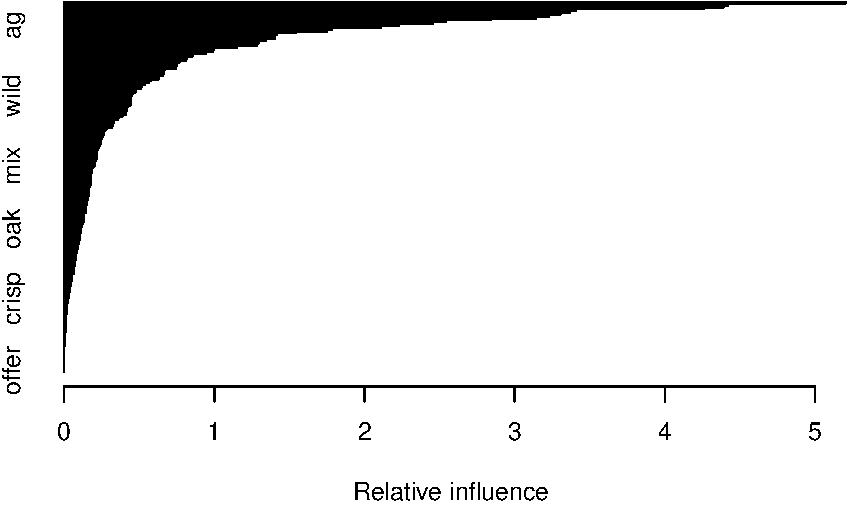
\includegraphics{thesis_files/figure-latex/unnamed-chunk-7-1.pdf}
\begin{verbatim}
             var  rel.inf
     1      rich 5.201027
     2  vineyard 4.417346
     3   complex 4.389741
     4     simpl 4.256652
     5  concentr 3.403552
     6     black 3.368652
     7      year 3.303258
     8      long 3.226283
     9     power 3.142659
     10     eleg 2.842253
\end{verbatim}
The word ``rich'' has the highest relative influence, followed by words
like ``vineyard,'' ``complex,'' the stemmed ``simpl,'' and the stemmed
``concentr.''

However, because the model with price, province, and variety included
has a lower MSE, and because these variables would not be difficult to
find for an average wine drinker, we will use the model with 500 trees
with price, province, and variety included to build our prediction
engine.

\chapter{Geocoding and Visualization}\label{geocoding-and-visualization}

\section{Why Geocode?}\label{why-geocode}

Geocoding locations is generally a good idea because it allows for
spatial analysis and spatial visualizations. In our case, geocoding the
wine reviews will allow us to create interactive maps that visualize the
wineries and allows users to explore our dataset.

\section{\texorpdfstring{Using
\texttt{ggmap}}{Using ggmap}}\label{using-ggmap}

The most convenient approach to perform geocoding in R is to use the
\texttt{ggmap} package. However, the rather recent change in Google's
API requires setting up a project and generating a key in the Google
Cloud Project. While we are billed for every observation that we
geocode, we have credits available each month. To find out more about
the API usage and billing refer to
\href{https://developers.google.com/maps/documentation/geocoding/usage-and-billing}{the
official website.} To learn more about the \texttt{ggmap} package check
out the \href{https://github.com/dkahle/ggmap}{project's Github
repository.}

\subsection{Reading in the Data}\label{reading-in-the-data}
\begin{Shaded}
\begin{Highlighting}[]
\NormalTok{data_dir <-}\StringTok{ "../data"}
\NormalTok{file_name <-}\StringTok{ "winemag-data-130k-v2.csv"}

\NormalTok{path <-}\StringTok{ }\KeywordTok{file.path}\NormalTok{(data_dir, file_name)}
\end{Highlighting}
\end{Shaded}
\begin{Shaded}
\begin{Highlighting}[]
\NormalTok{Wine <-}\StringTok{ }\KeywordTok{read_csv}\NormalTok{(path) }\OperatorTok\StringTok{ }
\StringTok{    }\KeywordTok{rename}\NormalTok{(}\DataTypeTok{id =}\NormalTok{ X1) }\OperatorTok\StringTok{ }
\StringTok{    }\KeywordTok{mutate}\NormalTok{(}\DataTypeTok{id =}\NormalTok{ id }\OperatorTok{+}\StringTok{ }\DecValTok{1}\NormalTok{) }
\end{Highlighting}
\end{Shaded}
The \texttt{mutate\_geocoded} function from \texttt{ggmap} would be
great if it actually had some error handling. However, it is not robust
enough for our needs. Instead, we will create our own function to handle
both network and API errors, while ensuring completion of our code.

We will operate in a small sample of observations. This will allow us to
test our function and then apply it to the whole dataset.
\begin{Shaded}
\begin{Highlighting}[]
\KeywordTok{set.seed}\NormalTok{(}\DecValTok{2019}\NormalTok{)}

\NormalTok{subset <-}\StringTok{ }\NormalTok{Wine }\OperatorTok
\StringTok{    }\KeywordTok{count}\NormalTok{(winery, country) }\OperatorTok
\StringTok{    }\KeywordTok{mutate}\NormalTok{(}\DataTypeTok{address =} \KeywordTok{paste0}\NormalTok{(winery, }\StringTok{" "}\NormalTok{, country)) }\OperatorTok
\StringTok{    }\KeywordTok{sample_n}\NormalTok{(}\DecValTok{20}\NormalTok{) }
\end{Highlighting}
\end{Shaded}
\subsection{Setting Up Helper
Function}\label{setting-up-helper-function}

We mentioned that the function we use to geocode our observations has to
be robust. We take advantage of the \texttt{purrr} adverbs to handle
internal messages that slow down the operation of the geocoding function
in \texttt{ggmap}. Additionally, we prevent network failures from being
an issue by allowing failed requests to retry at most once after a short
delay. Finally, in order to be able to ensure the completion of our code
without errors, we wrap the geocoding functionality with an alternative
for when the function fails.

You can see all these components working together in the function below.
\begin{Shaded}
\begin{Highlighting}[]
\NormalTok{geocode_robustly <-}
\StringTok{    }\KeywordTok{possibly}\NormalTok{(}
        \KeywordTok{insistently}\NormalTok{(}
            \KeywordTok{quietly}\NormalTok{(geocode),}
            \DataTypeTok{rate =} \KeywordTok{rate_delay}\NormalTok{(}\FloatTok{0.1}\NormalTok{, }\DataTypeTok{max_times =} \DecValTok{2}\NormalTok{)),}
        \DataTypeTok{otherwise =} \KeywordTok{list}\NormalTok{(}\DataTypeTok{result =} \KeywordTok{tibble}\NormalTok{(}\DataTypeTok{lon =} \OtherTok{NA_real_}\NormalTok{, }\DataTypeTok{lat =} \OtherTok{NA_real_}\NormalTok{))}
\NormalTok{    )}
\end{Highlighting}
\end{Shaded}
It is important to make sure that the \texttt{otherwise} argument
matches the type of output given by the function that is wrapped by the
\texttt{possibly} adverb.

Finally, we apply our function to the addresses of the observations.
\begin{Shaded}
\begin{Highlighting}[]
\NormalTok{locations <-}\StringTok{ }\NormalTok{subset }\OperatorTok
\StringTok{    }\KeywordTok{pull}\NormalTok{(address) }\OperatorTok
\StringTok{    }\KeywordTok{map_dfr}\NormalTok{(}\OperatorTok{~}\StringTok{ }\KeywordTok{geocode_robustly}\NormalTok{(.x)}\OperatorTok{$}\NormalTok{result)}

\NormalTok{subset }\OperatorTok\StringTok{ }\KeywordTok{bind_cols}\NormalTok{(locations)}
\end{Highlighting}
\end{Shaded}
Note that there will be some \texttt{NA} values in our location
variables because we are largely relying on the integrity of the dataset
and the Google Maps search engine.

Confirming that our function is operating as desired, we can now we
geocode all the units in our dataset.

\subsection{Putting It All Together}\label{putting-it-all-together}

In the code below we perform a further optimization by only geocoding
the set of wineries. This allows us to avoid performing slow network
requests on observations that have already been geocoded. The following
represents every step taken to geocode our dataset with more than 100K
observations. (The code will take some time to run.)
\begin{Shaded}
\begin{Highlighting}[]
\CommentTok{# 1. Add address column to geocode}
\NormalTok{Wine <-}\StringTok{ }\NormalTok{Wine }\OperatorTok
\StringTok{    }\KeywordTok{mutate}\NormalTok{(}\DataTypeTok{address =} \KeywordTok{paste0}\NormalTok{(winery, }\StringTok{" "}\NormalTok{, country))}

\CommentTok{# 2. Get unique addresses}
\NormalTok{Addresses <-}\StringTok{ }\NormalTok{Wine }\OperatorTok
\StringTok{    }\KeywordTok{count}\NormalTok{(address) }\OperatorTok
\StringTok{    }\KeywordTok{select}\NormalTok{(}\OperatorTok{-}\NormalTok{n)}

\CommentTok{# 3. Geocode unique addresses}
\NormalTok{Locations <-}\StringTok{ }\NormalTok{Addresses }\OperatorTok
\StringTok{    }\KeywordTok{pull}\NormalTok{(address) }\OperatorTok
\StringTok{    }\KeywordTok{map_dfr}\NormalTok{(}\OperatorTok{~}\StringTok{ }\KeywordTok{geocode_robustly}\NormalTok{(.x)}\OperatorTok{$}\NormalTok{result)}

\CommentTok{# 4. Bind location info to addresses}
\NormalTok{Addresses <-}\StringTok{ }\NormalTok{Addresses }\OperatorTok
\StringTok{    }\KeywordTok{bind_cols}\NormalTok{(Locations) }

\CommentTok{# 5. Join into original dataset}
\NormalTok{Geocoded_Wine <-}\StringTok{ }\NormalTok{Wine }\OperatorTok
\StringTok{    }\KeywordTok{left_join}\NormalTok{(Addresses, }\DataTypeTok{by =} \StringTok{"address"}\NormalTok{)}

\CommentTok{# 4. Save geocoded dataset}
\NormalTok{file_name <-}\StringTok{ "geocoded.csv.gz"}
\NormalTok{Geocoded_Wine }\OperatorTok\StringTok{ }\KeywordTok{write_csv}\NormalTok{(}\DataTypeTok{path =} \KeywordTok{file.path}\NormalTok{(data_dir, file_name))}
\end{Highlighting}
\end{Shaded}
Now we have a geocoded version of the dataset that we can further refine
for our analysis.

\section{Verify}\label{verify}

To prove that our geocoding worked we can import our new dataset.
\begin{Shaded}
\begin{Highlighting}[]
\NormalTok{Wine <-}\StringTok{ }\KeywordTok{read_csv}\NormalTok{(}\StringTok{"../data/geocoded.csv.gz"}\NormalTok{) }\OperatorTok
\StringTok{    }\KeywordTok{glimpse}\NormalTok{()}
\end{Highlighting}
\end{Shaded}
\begin{verbatim}
     Observations: 129,971
     Variables: 17
     $ id                    <dbl> 1, 2, 3, 4, 5, 6, 7, 8, 9, 10, 11, 12, 1...
     $ country               <chr> "Italy", "Portugal", "US", "US", "US", "...
     $ description           <chr> "Aromas include tropical fruit, broom, b...
     $ designation           <chr> "Vulkà Bianco", "Avidagos", NA, "Reserve...
     $ points                <dbl> 87, 87, 87, 87, 87, 87, 87, 87, 87, 87, ...
     $ price                 <dbl> NA, 15, 14, 13, 65, 15, 16, 24, 12, 27, ...
     $ province              <chr> "Sicily & Sardinia", "Douro", "Oregon", ...
     $ region_1              <chr> "Etna", NA, "Willamette Valley", "Lake M...
     $ region_2              <chr> NA, NA, "Willamette Valley", NA, "Willam...
     $ taster_name           <chr> "Kerin O’Keefe", "Roger Voss", "Paul Gre...
     $ taster_twitter_handle <chr> "@kerinokeefe", "@vossroger", "@paulgwin...
     $ title                 <chr> "Nicosia 2013 Vulkà Bianco  (Etna)", "Qu...
     $ variety               <chr> "White Blend", "Portuguese Red", "Pinot ...
     $ winery                <chr> "Nicosia", "Quinta dos Avidagos", "Rains...
     $ address               <chr> "Nicosia Italy", "Quinta dos Avidagos Po...
     $ lon                   <dbl> 14.395278, -7.276971, -95.712891, -85.89...
     $ lat                   <dbl> 37.74692, 41.38793, 37.09024, 42.21225, ...
\end{verbatim}
\section{Building Our Shiny App}\label{building-our-shiny-app}

Our Shiny app can be found
\href{https://szablah.shinyapps.io/wine/}{here}. There are 3 components:
first, an interactive map that allows users to view wineries of the
world and filter based on variety. Users can see average points or
average price of the wines around the world. The second component of the
Shiny app is a searchable catalog, where users can search among any of
the wines included in the catalog and geolocate them on the map. The
third and final component of our Shiny app is a prediction engine, which
allows users to input their own wine with country, province,
description, price, and variety, and our prediction model described in
the previous chapter will produce an estimate of the number of points
the inputted wine would receive.

\chapter*{Conclusion}\label{conclusion}
\addcontentsline{toc}{chapter}{Conclusion}

This project set out to make wine easier to understand for the average
person. Through this project, we examined close to 130,000 wine reviews
to create a complex web application via Shiny that allows users to
explore wines and wineries through an interactive map and searchable
catalog as well as to enter new wine observations to receive a
prediction of how many point values their new wine would receive.
Through the map and catalog explorer and prediction engine, anyone can
learn more about wine and explore the different varieties around the
world.

This project also involved text analysis beyond the scope of our
Stat-495 class, researching into word ranking methods such as term
frequency-inverse document frequency and learning how to incorporate
document-term matrices into our prediction model. Our gradient boosting
model showed that the most important features to predicting wine points
are price, variety, and province. The most important word for prediction
is ``rich.''

\section{Limitations and Future
Directions}\label{limitations-and-future-directions}

There were several limitations to the work in this project. They will be
discussed below, and various suggestions for future directions to
address these limitations will be described.

\subsection{Data Scraping}\label{data-scraping}

The Kaggle dataset we used originated from Wine Magazine's website and
was scraped in 2017. However, in the most recent years, almost 100,000
more wines have been added to the website. A future direction this
project could go into would be to use the python scraper provided by the
Kaggle user who uploaded the original dataset\footnote{Thoutt (2017)}
and scrape the newer wine reviews so there would be more up-to-date
data.

\subsection{Model Computation Run
Time}\label{model-computation-run-time}

A key limitation to the prediction aspect of this project was the sheer
amount of computation involved. The model created in this project used
only 200 of the words with the highest mean TF-IDF values, but models
with many more words could have been created and would likely yield
lower MSE values and better predictions. However, given how the gradient
boosting algorithm is computationally intensive because it requires
creating many small trees, we chose to limit the number of variables
used in the dataset to run the model.

Future steps that could be made in order to speed up computation time
and create a more accurate model could be to look into faster gradient
boosting algorithm methods. In R, there are newer packages such as
\texttt{XGBoost} and \texttt{LightGBM} that were developed specifically
for decreasing run time of the computationally intensive gradient
boosting algorithms, so the functions in these packages could be
explored on the data in this project.

\subsection{Confirmation Bias}\label{confirmation-bias}

Although our analyses were run on the assumption that there was no bias
among tasters who were rating wine points, we do not know how the
original data was collected and whether the tasters were blind to
various aspects about the wine they were tasting (for example, price or
variety). It is possible that the reason the positive correlation
between points and price was acually due to confirmation bias among
tasters that more expensive wine should taste better. An interesting
further direction this project could go in would be to explore whether
different tasters had different patterns of rating wines to possibly
discern if these tasters were biased.

\backmatter

\chapter*{References}\label{references}
\addcontentsline{toc}{chapter}{References}

\markboth{References}{References}

\noindent

\setlength{\parindent}{-0.20in} \setlength{\leftskip}{0.20in}
\setlength{\parskip}{8pt}

\hypertarget{refs}{}
\hypertarget{ref-ho2018}{}
Ho, S. (2018, April). Document-term matrix: Text mining in r and python.
Retrieved from
\url{https://towardsdatascience.com/machine-learning-text-processing-1d5a2d638958}

\hypertarget{ref-jones2019}{}
Jones, T. (2018). TextmineR vignette. Retrieved from
\url{https://cran.r-project.org/web/packages/textmineR/vignettes/a_start_here.html}

\hypertarget{ref-manning2008}{}
Manning, C. D., Raghavan, P., \& Schütze, H. (2008). \emph{Introduction
to information retrieval}. Boston, MA: Cambridge University Press.

\hypertarget{ref-textprocess}{}
Nabi, J. (2018, September). Machine learning - text processing.
Retrieved from
\url{https://towardsdatascience.com/machine-learning-text-processing-1d5a2d638958}

\hypertarget{ref-kagglepredict}{}
Predicting wine ratings using lightgbm + text2vec. (2018). Retrieved
from
\url{https://www.kaggle.com/nnnnick/predicting-wine-ratings-using-lightgbm-text2vec}

\hypertarget{ref-thoutt2017}{}
Thoutt, Z. (2017). Wine reviews. Retrieved from
\url{https://www.kaggle.com/zynicide/wine-reviews}

\hypertarget{ref-watson2010}{}
Watson, I. (2010, April). Unearthing georgia's wine heritage. Retrieved
from
\url{http://edition.cnn.com/2010/WORLD/europe/04/20/georgia.wine.heritage/}

\hypertarget{ref-winemag}{}
Wine enthusiast reviews. (2019). Retrieved from
\url{https://www.winemag.com/?s=\&drink_type=wine\&page=0}


% Index?

\end{document}
